% RECALL — english-vocabulary vault, practice set 4: comeback review (answer key)
% Compile with: pdflatex vocabulary-answers-4.tex  (run twice)

\documentclass[11pt,a4paper]{article}
\usepackage[T1]{fontenc}
\usepackage[utf8]{inputenc}
\usepackage{charter}
\usepackage[scaled=0.92]{helvet}
\usepackage{courier}
\usepackage[safe]{tipa}
\usepackage{amssymb}
\usepackage{pifont}
\usepackage[a4paper,left=17mm,right=17mm,top=21mm,bottom=19mm,headsep=6mm,footskip=10mm]{geometry}
\usepackage{xcolor}
\usepackage{tikz}
\usetikzlibrary{calc,positioning,arrows.meta,backgrounds,shapes.geometric,shapes.misc,fit,decorations.pathreplacing,decorations.pathmorphing}
\usepackage[most]{tcolorbox}
\usepackage{enumitem}
\usepackage{multicol}
\usepackage{tabularx}
\usepackage{array}
\usepackage{booktabs}
\usepackage{colortbl}
\usepackage{fancyhdr}
\makeatletter
\newcommand{\needsp}[1]{\par\begingroup\setlength{\dimen@}{#1}\dimen@ii\pagegoal\advance\dimen@ii-\pagetotal
  \ifdim\dimen@>\dimen@ii\ifdim\dimen@ii>\z@\vfil\penalty-\@M\fi\fi\endgroup}
\makeatother
\raggedbottom
\usepackage{microtype}
\usepackage{etoolbox}
\usepackage{ragged2e}
\usepackage[hidelinks,pdftitle={Recall - Vocabulary vault comeback (answer key)},pdfauthor={FHX}]{hyperref}

% ---------- colours ----------
\definecolor{ink}{HTML}{1F2633}
\definecolor{inksoft}{HTML}{4A5466}
\definecolor{mute}{HTML}{8A93A3}
\definecolor{line}{HTML}{C3C9D4}
\definecolor{paper}{HTML}{F1F4F7}
\definecolor{accent}{HTML}{1C86C8}
\definecolor{accentdark}{HTML}{145E8E}
\definecolor{accentsoft}{HTML}{E3F0F9}
\definecolor{vault}{HTML}{E09F3E}
\definecolor{vaultsoft}{HTML}{FBF0DF}
\definecolor{good}{HTML}{2E8B57}
\definecolor{bad}{HTML}{C0392B}
% media colours (the shows your words came from)
\definecolor{mDB}{HTML}{E07A1F}
\definecolor{mJJK}{HTML}{6A4FC2}
\definecolor{mMHA}{HTML}{2E7D5B}
\definecolor{mMT}{HTML}{B5509A}
\definecolor{mDS}{HTML}{7A9A1F}
\definecolor{mPB}{HTML}{5A6170}
\definecolor{mFI}{HTML}{C8302C}
\definecolor{mLF}{HTML}{B07D12}
% voices (casters, chats)
\definecolor{vA}{HTML}{3A86C8}
\definecolor{vB}{HTML}{D1495B}

% ---------- fonts ----------
\newcommand{\mdot}{\ensuremath{\cdot}}
\newcommand{\arr}{\ensuremath{\rightarrow}}
\newcommand{\hfont}{\fontfamily{pag}\selectfont}
\newcommand{\uifont}{\sffamily}
\setlength{\parindent}{0pt}
\setlength{\parskip}{4pt}
\linespread{1.04}
\setlist{nosep,leftmargin=*}
\renewcommand{\arraystretch}{1.15}

% ---------- small TikZ icons (drawn in mm, centred on 0,0) ----------
\tikzset{
  ic/.style={x=1mm,y=1mm,line width=0.5pt,line join=round,line cap=round},
  pics/pencil/.style={code={
    \begin{scope}[rotate=40]
    \fill (-1.45,-0.32) rectangle (0.75,0.32);
    \fill (0.85,-0.32) -- (1.55,0) -- (0.85,0.32) -- cycle;
    \end{scope}}},
  pics/bubble/.style={code={
    \fill[rounded corners=0.55mm] (-1.5,-0.55) rectangle (1.5,1.05);
    \fill (-0.75,-0.45) -- (-1.05,-1.35) -- (-0.1,-0.45) -- cycle;}},
  pics/watch/.style={code={
    \draw (0,-0.2) circle (1.12);
    \fill (-0.28,0.95) rectangle (0.28,1.4);
    \draw (0,-0.2) -- (0,0.5);
    \draw (0,-0.2) -- (0.45,-0.2);}},
  pics/lens/.style={code={
    \draw[line width=0.62pt] (-0.35,0.35) circle (0.85);
    \draw[line width=1pt] (0.28,-0.28) -- (1.25,-1.25);}},
  pics/die/.style={code={
    \draw[rounded corners=0.35mm,line width=0.55pt] (-1.25,-1.25) rectangle (1.25,1.25);
    \fill (-0.6,0.6) circle (0.24); \fill (0.6,-0.6) circle (0.24); \fill (0,0) circle (0.24);}},
  pics/rewind/.style={code={
    \fill (-0.1,0) -- (1.3,0.95) -- (1.3,-0.95) -- cycle;
    \fill (-1.5,0) -- (-0.1,0.95) -- (-0.1,-0.95) -- cycle;}},
  pics/key/.style={code={
    \draw[line width=0.62pt] (-0.85,0.3) circle (0.62);
    \draw[line width=0.62pt] (-0.23,0.3) -- (1.55,0.3);
    \draw[line width=0.62pt] (1.05,0.3) -- (1.05,-0.35);
    \draw[line width=0.62pt] (1.5,0.3) -- (1.5,-0.2);}},
}
% mode icons: plain ink glyphs
\newcommand{\modeicon}[1]{\tikz[ic,baseline=-0.65ex]{\path (-1.9,-1.9) rectangle (1.9,1.9); \pic[inksoft] at (0,0) {#1};}}
\newcommand{\mWrite}{\modeicon{pencil}}
\newcommand{\mSpeak}{\modeicon{bubble}}
\newcommand{\mThink}{\modeicon{lens}}
\newcommand{\mTimed}{\modeicon{watch}}
\newcommand{\mDice}{\modeicon{die}}
% language chips
\newcommand{\langchip}[2]{\tikz[baseline=(c.base)]{\node[inner xsep=2.2pt,inner ysep=1.3pt,rounded corners=1.2pt,fill=#1,text=white,font=\uifont\bfseries\fontsize{6.2}{7}\selectfont](c){#2};}}
\newcommand{\PT}{\langchip{good}{PT}}
\newcommand{\UK}{\langchip{bad!85!ink}{UK}}
\newcommand{\US}{\langchip{accentdark}{US}}
% vault key marker
\newcommand{\vaultI}{\tikz[ic,baseline=-0.65ex]{\fill[vault] (0,0) circle (2.2); \pic[white,scale=0.85] at (0,0) {key};}}

% media chips: #1 colour, #2 label
\newcommand{\medchip}[2]{\tikz[baseline=(c.base)]{\node[inner xsep=1.8pt,inner ysep=0.9pt,rounded corners=1pt,fill=#1,text=white,font=\uifont\bfseries\fontsize{5.6}{6}\selectfont](c){#2};}}
\newcommand{\mDBZ}{\medchip{mDB}{DBZ}}
\newcommand{\mDBS}{\medchip{mDB}{DBS}}
\newcommand{\mGT}{\medchip{mDB}{GT}}
\newcommand{\mJJK}{\medchip{mJJK}{JJK}}
\newcommand{\mMHA}{\medchip{mMHA}{MHA}}
\newcommand{\mMT}{\medchip{mMT}{MT}}
\newcommand{\mDS}{\medchip{mDS}{DS}}
\newcommand{\mPB}{\medchip{mPB}{PB}}
\newcommand{\mFI}{\medchip{mFI}{F1}}
\newcommand{\mLF}{\medchip{mLF}{LIFE}}

% ---------- slanted label (Overwatch-HUD style parallelogram) ----------
% #1 half-slant, #2 fill colour, #3 node options, #4 text
\newcommand{\slant}[4][2.2pt]{\tikz[baseline=(t.base)]{\node[inner xsep=5pt,inner ysep=2.4pt,#3](t){#4};
  \begin{scope}[on background layer]\fill[#2]($(t.south west)+(-#1,0)$)--($(t.south east)+(-#1,0)$)--($(t.north east)+(#1,0)$)--($(t.north west)+(#1,0)$)--cycle;\end{scope}}}
% knowledge tags
\newcommand{\tg}[1]{\slant[1.5pt]{ink!9}{font=\hfont\bfseries\scriptsize,text=inksoft,inner xsep=3.2pt,inner ysep=1.6pt}{#1}}
\newcommand{\tgA}[1]{\slant[1.3pt]{ink!8}{font=\hfont\bfseries\tiny,text=inksoft,inner xsep=2.3pt,inner ysep=1.2pt}{#1}}
\newcommand{\tgL}[2]{\slant[1.5pt]{ink!9}{font=\hfont\scriptsize,text=inksoft,inner xsep=3.2pt,inner ysep=1.6pt}{\textbf{#1}\,{\color{mute}·}\,#2}}
\newcommand{\exnum}[1]{\slant[3pt]{accent}{font=\hfont\bfseries\fontsize{19}{19}\selectfont,text=white,inner xsep=7pt,inner ysep=5pt,minimum height=10.5mm}{#1}}

% ---------- headers / footers ----------
\setlength{\headheight}{14pt}
\pagestyle{fancy}
\fancyhf{}
\renewcommand{\headrulewidth}{0.4pt}
\renewcommand{\headrule}{{\color{line}\hrule height 0.4pt}}
\fancyhead[L]{{\hfont\bfseries\footnotesize\color{accent}RECALL}{\hfont\footnotesize\color{mute}\ \ \mdot{}\ \ Vocabulary vault comeback}}
\fancyhead[R]{{\hfont\footnotesize\color{mute}Answer key}}
\fancyfoot[R]{\slant[2pt]{ink}{font=\hfont\bfseries\footnotesize,text=white,inner xsep=6pt}{\thepage}}
\fancyfoot[L]{{\hfont\scriptsize\color{mute}english-vocabulary vault \mdot{}\ Practice set 4}}
\fancypagestyle{plain}{\fancyhf{}\renewcommand{\headrulewidth}{0pt}\fancyfoot[R]{\slant[2pt]{ink}{font=\hfont\bfseries\footnotesize,text=white,inner xsep=6pt}{\thepage}}}

% ---------- part banner ----------
% #1 part label, #2 title, #3 subtitle
\newcommand{\partbanner}[3]{%
  \needsp{100mm}\vspace{6mm}
  \noindent\begin{tikzpicture}
    \path[use as bounding box] (0,0) rectangle (\linewidth,-21.5mm);
    \fill[ink] (0,0) -- (\linewidth,0) -- (\linewidth-9mm,-15mm) -- (0,-15mm) -- cycle;
    \fill[accent] (0,0) rectangle (3.2mm,-15mm);
    \fill[accent] (\linewidth-5mm,0) -- (\linewidth,0) -- (\linewidth-9mm,-15mm) -- (\linewidth-14mm,-15mm) -- cycle;
    \fill[vault] (\linewidth-12mm,0) -- (\linewidth-9.6mm,0) -- (\linewidth-18.6mm,-15mm) -- (\linewidth-21mm,-15mm) -- cycle;
    \node[anchor=west,font=\hfont\bfseries\footnotesize,text=accent!70!white] at (7.5mm,-4.6mm) {#1};
    \node[anchor=west,font=\hfont\bfseries\fontsize{21}{23}\selectfont,text=white] at (7mm,-10.3mm) {#2};
    \node[anchor=north west,font=\itshape\small,text=inksoft,inner sep=0pt] at (0.4mm,-17.6mm) {#3};
  \end{tikzpicture}\par\vspace{1mm}}

% ---------- exercise header ----------
% #1 number, #2 title, #3 tag pills, #4 icons
\newcommand{\exhead}[5][10\baselineskip]{%
  \needsp{#1}\vspace{9pt}%
  \noindent\begin{tikzpicture}[baseline=(n.south)]
    \node[anchor=south west,inner sep=0pt] (n) at (0,0) {\exnum{#2}};
    \node[anchor=south west,inner sep=0pt,font=\hfont\bfseries\fontsize{14.5}{16}\selectfont,text=ink] (t) at ($(n.south east)+(4mm,4.8mm)$) {#3};
    \node[anchor=south west,inner sep=0pt] (u) at ($(n.south east)+(4mm,0.1mm)$) {#4};
    \node[anchor=south east,inner sep=0pt] (i) at (\linewidth-0.3pt,1.2mm) {#5};
    \draw[line,line width=0.6pt] (0.3pt,-1.6mm) -- (\linewidth-0.3pt,-1.6mm);
  \end{tikzpicture}\par\vspace{3pt}}
\newcommand{\instr}[1]{{\small\color{inksoft}#1}\par\vspace{2pt}}

% ---------- gaps, options, writing lines ----------
% #1 number, #2 width, #3 hint
\newcommand{\gap}[3]{\mbox{{\uifont\bfseries\scriptsize\color{accent}#1}\kern1.2pt\textcolor{mute}{\rule[-0.5ex]{#2}{0.5pt}}}\ifstrempty{#3}{}{\ ({\itshape #3})}}
\newcommand{\opt}[2]{\mbox{{\color{mute}[}\,{\uifont\small #1}~{\color{mute}/}~{\uifont\small #2}\,{\color{mute}]}}}
\newcommand{\optt}[3]{\mbox{{\color{mute}[}\,{\uifont\small #1}~{\color{mute}/}~{\uifont\small #2}~{\color{mute}/}~{\uifont\small #3}\,{\color{mute}]}}}
\newcommand{\wfill}{\leavevmode{\color{line}\leaders\hrule height 0.5pt\hfill\kern0pt}}
\newcommand{\wline}{\par\vspace{5.6mm}\noindent{\color{line}\rule{\linewidth}{0.5pt}}\par}
\newcommand{\wlines}[1]{\foreach\x in {1,...,#1}{\wline}\vspace{1mm}}
\newcommand{\num}[1]{\leavevmode{\uifont\bfseries\small\color{accent}#1}}
\newcommand{\blank}[1][1.25cm]{\textcolor{mute}{\rule[-0.45ex]{#1}{0.5pt}}}
\newcommand{\cbox}{\tikz[baseline=-0.75ex]{\draw[mute,line width=0.5pt,rounded corners=0.4pt] (0,-1.35mm) rectangle (2.7mm,1.35mm);}}
\newcommand{\lbox}[1]{\tikz[baseline=-0.75ex]{\draw[mute,line width=0.5pt,rounded corners=0.4pt] (0,-1.6mm) rectangle (#1,1.6mm);}}
\newcommand{\hl}[1]{{\uifont\bfseries #1}}
\newcommand{\sout}[1]{\tikz[baseline=(t.base)]{\node[inner sep=0pt,text=inksoft](t){#1}; \draw[bad,line width=0.7pt] ([xshift=-0.4pt]t.mid west) -- ([xshift=0.4pt]t.mid east);}}
\newcommand{\ul}[1]{\underline{#1}}
\newcommand{\word}[1]{{\uifont\bfseries\color{ink}#1}}

% ---------- boxes ----------
\newtcolorbox{infobox}[2][]{enhanced,breakable,colback=paper,colframe=paper,boxrule=0pt,arc=2mm,left=4mm,right=4mm,top=3mm,bottom=3mm,
  fonttitle=\hfont\bfseries\small,coltitle=ink,title={#2},attach title to upper={\par\vspace{2pt}},#1}
\newtcolorbox{vocabbox}[2][]{enhanced,breakable,colback=white,colframe=#1,boxrule=0.6pt,arc=2mm,left=4mm,right=4mm,top=2.5mm,bottom=2.5mm,
  fonttitle=\hfont\bfseries\small,coltitle=#1,title={#2},attach title to upper={\par\vspace{1pt}},fontupper=\small}
\newtcolorbox{speakbox}[1][]{enhanced,breakable,colback=accentsoft,colframe=accentsoft,boxrule=0pt,arc=2mm,left=4mm,right=4mm,top=2.5mm,bottom=2.5mm,
  fontupper=\small,#1}
\newtcolorbox{vaultbox}[1][]{enhanced,breakable,colback=vaultsoft,colframe=vaultsoft,boxrule=0pt,arc=2mm,left=4mm,right=4mm,top=2.5mm,bottom=2.5mm,
  fontupper=\small,#1}
\newcommand{\banksep}{}
\newcommand{\bankitem}[1]{\banksep\mbox{#1}\gdef\banksep{\nobreak\hspace{0.5em plus 0.3em}{\color{mute}\mdot}\nobreak\hspace{0.5em plus 0.3em}\allowbreak}}
\newcommand{\bank}[1]{\gdef\banksep{}\forcsvlist{\bankitem}{#1}}
\newtcolorbox{wordbank}[1][]{enhanced,colback=white,colframe=line,boxrule=0.5pt,arc=1.5mm,left=3mm,right=3mm,top=1.6mm,bottom=1.6mm,
  fontupper=\small\uifont,halign=center,#1}

\newcommand{\ai}[3]{\par\noindent\hangindent=6mm\hangafter=1\makebox[6mm][l]{\num{#1}}#2\nobreak\hfill\nobreak\mbox{#3}\par}
\newcommand{\an}[1]{\par\noindent\hspace*{6mm}\parbox[t]{\dimexpr\linewidth-6mm\relax}{\footnotesize\itshape\color{inksoft}\RaggedRight #1}\par\vspace{1.5pt}}
\newcommand{\akhead}[4][7\baselineskip]{\needsp{#1}\vspace{8pt}\noindent
  \slant[2.4pt]{accent}{font=\hfont\bfseries\normalsize,text=white,inner xsep=6pt,inner ysep=3.2pt}{#2}\hspace{3mm}{\hfont\bfseries\large\color{ink}#3}\hfill#4\par
  \vspace{1pt}{\color{line}\hrule height 0.5pt}\vspace{4pt}}
\newcommand{\why}[1]{{\footnotesize\itshape\color{inksoft}#1}\par}
\newenvironment{aitem}{\par\noindent\begin{minipage}[t]{\linewidth}\RaggedRight}{\end{minipage}\par\vspace{1.2pt}}
\newcommand{\ipa}[1]{{\fontfamily{cmr}\fontseries{m}\fontshape{n}\selectfont\textipa{#1}}}
\newcommand{\badge}[2]{\tikz[baseline=(c.base)]{\node[inner xsep=2pt,inner ysep=1pt,rounded corners=1pt,fill=#1,text=white,font=\uifont\bfseries\fontsize{5.6}{6}\selectfont](c){#2};}}
\newcommand{\newsense}{\badge{good}{+ NOT ON YOUR CARD}}
\newcommand{\vfix}{\badge{vault}{VAULT FIX}}
\newcommand{\gl}[3]{\par{\RaggedRight\noindent\hangindent=4mm\hangafter=1{\uifont\bfseries\small #1}\enspace{\small\color{inksoft}#2}\nobreak\hfill\nobreak\mbox{#3}\par}\vspace{0.8pt}}
\newcommand{\lab}[1]{{\upshape\uifont\bfseries\color{accent}#1}}
\newcommand{\sub}[1]{\par\vspace{2pt}\noindent{\hfont\bfseries\small\color{accent}#1}\par\vspace{1pt}}
\newcommand{\model}[1]{\begin{tcolorbox}[enhanced,breakable,colback=paper,colframe=paper,boxrule=0pt,arc=1.5mm,left=3.5mm,right=3.5mm,top=2mm,bottom=2mm,fontupper=\small]#1\end{tcolorbox}}

\begin{document}

\thispagestyle{plain}
\noindent
\begin{tikzpicture}
  \path[use as bounding box] (0,0) rectangle (\linewidth,-30mm);
  \fill[ink] (0,0) -- (\linewidth,0) -- (\linewidth-10mm,-26mm) -- (0,-26mm) -- cycle;
  \fill[accent] (\linewidth-5mm,0) -- (\linewidth,0) -- (\linewidth-10mm,-26mm) -- (\linewidth-15mm,-26mm) -- cycle;
  \fill[vault] (\linewidth-12mm,0) -- (\linewidth-9.5mm,0) -- (\linewidth-19.5mm,-26mm) -- (\linewidth-22mm,-26mm) -- cycle;
  \fill[accent] (0,0) rectangle (3.4mm,-26mm);
  \node[anchor=west,font=\hfont\bfseries\footnotesize,text=accent!75!white] at (8.5mm,-6.5mm) {ENGLISH-VOCABULARY VAULT \enspace\mdot{}\enspace PRACTICE SET 4};
  \node[anchor=west,font=\hfont\bfseries\fontsize{30}{32}\selectfont,text=white] (rs) at (7.5mm,-16.5mm) {RECALL};
  \node[anchor=base west,font=\hfont\bfseries\fontsize{19}{21}\selectfont,text=accent] at ([xshift=4mm]rs.base east) {ANSWER KEY};
\end{tikzpicture}
\par\vspace{1mm}
\begin{infobox}{HOW TO CHECK}
\textbf{Bold} = the expected answer; {\color{inksoft}grey after a slash} = also correct. Mark every answer in your colours (blue / orange / red) and, for every red, colour one square next to its tag (\tgA{S}, \tgA{C}\ldots) on the \emph{Rundown} page. Chips like \mJJK\,{\uifont\fontsize{5.4}{6}\selectfont\color{mute}MAR} tell you which show and which month the card comes from — open it after a mistake. \newsense{} = a meaning or fact your card is missing (worth adding). \vfix{} = something on your card that needs correcting; they are all collected at the end. \UK{} marks the British choice.
\end{infobox}

% ===================================================================== PART 1
\akhead{1}{Vault scan}{\tgA{M}}
\why{A \ding{51} only scores if your meaning matches. Then shade the bars on the exercise page and compare A (drilled in January) with C (never drilled).}
\noindent\begin{minipage}[t]{0.485\linewidth}
\sub{A \enspace JANUARY \enspace (drilled)}
\gl{withstand}{resist without being damaged}{\mDBZ\,{\uifont\fontsize{5.4}{6}\selectfont\color{mute}JAN}}
\gl{shrewd}{clever at judging situations}{\mDBZ\,{\uifont\fontsize{5.4}{6}\selectfont\color{mute}JAN}}
\gl{ominous}{suggesting something bad is coming}{\mDBZ\,{\uifont\fontsize{5.4}{6}\selectfont\color{mute}JAN}}
\gl{ponder}{think carefully for a long time}{\mDBZ\,{\uifont\fontsize{5.4}{6}\selectfont\color{mute}JAN}}
\gl{grudge}{resentment that lasts for years}{\mDBZ\,{\uifont\fontsize{5.4}{6}\selectfont\color{mute}JAN}}
\gl{ample}{enough, or more than enough}{\mDBZ\,{\uifont\fontsize{5.4}{6}\selectfont\color{mute}JAN}}
\gl{insidious}{spreading unnoticed, but harmful}{\mDBZ\,{\uifont\fontsize{5.4}{6}\selectfont\color{mute}JAN}}
\gl{thereby}{as a result of this (formal)}{\mDBZ\,{\uifont\fontsize{5.4}{6}\selectfont\color{mute}JAN}}
\gl{uncanny}{strange in a slightly scary way}{\mDBZ\,{\uifont\fontsize{5.4}{6}\selectfont\color{mute}JAN}}
\gl{loom}{appear large; be about to happen}{\mDBZ\,{\uifont\fontsize{5.4}{6}\selectfont\color{mute}JAN}}
\gl{brazen}{shamelessly bold}{\mDBZ\,{\uifont\fontsize{5.4}{6}\selectfont\color{mute}JAN}}
\gl{jeopardise}{put at risk}{\mDBZ\,{\uifont\fontsize{5.4}{6}\selectfont\color{mute}JAN}}
\end{minipage}\hfill\begin{minipage}[t]{0.485\linewidth}
\sub{B \enspace FEBRUARY}
\gl{breach}{break a rule; a gap in a defence}{\mJJK\,{\uifont\fontsize{5.4}{6}\selectfont\color{mute}FEB}}
\gl{deterrent}{something that discourages}{\mJJK\,{\uifont\fontsize{5.4}{6}\selectfont\color{mute}FEB}}
\gl{withhold}{refuse to give (info, payment)}{\mJJK\,{\uifont\fontsize{5.4}{6}\selectfont\color{mute}FEB}}
\gl{strive}{try very hard (for / to do)}{\mJJK\,{\uifont\fontsize{5.4}{6}\selectfont\color{mute}FEB}}
\gl{entrust}{hand over responsibility for}{\mJJK\,{\uifont\fontsize{5.4}{6}\selectfont\color{mute}FEB}}
\gl{plummet}{fall suddenly and steeply}{\mJJK\,{\uifont\fontsize{5.4}{6}\selectfont\color{mute}FEB}}
\gl{subtle}{hard to notice; clever, indirect}{\mJJK\,{\uifont\fontsize{5.4}{6}\selectfont\color{mute}FEB}}
\gl{ward off}{keep danger or illness away}{\mJJK\,{\uifont\fontsize{5.4}{6}\selectfont\color{mute}FEB}}
\gl{stir up}{deliberately cause trouble}{\mJJK\,{\uifont\fontsize{5.4}{6}\selectfont\color{mute}FEB}}
\gl{slack off}{work less hard than you should}{\mJJK\,{\uifont\fontsize{5.4}{6}\selectfont\color{mute}FEB}}
\gl{call it quits}{stop doing it; give up}{\mJJK\,{\uifont\fontsize{5.4}{6}\selectfont\color{mute}FEB}}
\gl{heirloom}{object passed down in a family}{\mJJK\,{\uifont\fontsize{5.4}{6}\selectfont\color{mute}FEB}}
\end{minipage}
\par\vspace{2mm}\needsp{60mm}
\noindent\begin{minipage}[t]{0.485\linewidth}
\sub{C \enspace MARCH \enspace (the 644)}
\gl{cope}{deal with difficulty (cope with)}{\mDBZ\,{\uifont\fontsize{5.4}{6}\selectfont\color{mute}MAR}}
\gl{convey}{communicate an idea or feeling}{\mJJK\,{\uifont\fontsize{5.4}{6}\selectfont\color{mute}MAR}}
\gl{deem}{consider, judge (formal)}{\mJJK\,{\uifont\fontsize{5.4}{6}\selectfont\color{mute}MAR}}
\gl{gauge}{measure or estimate; judge a mood}{\mJJK\,{\uifont\fontsize{5.4}{6}\selectfont\color{mute}MAR}}
\gl{heed}{pay attention to advice}{\mJJK\,{\uifont\fontsize{5.4}{6}\selectfont\color{mute}MAR}}
\gl{hindrance}{something that slows progress}{\mJJK\,{\uifont\fontsize{5.4}{6}\selectfont\color{mute}MAR}}
\gl{oblivious}{not aware (oblivious to / of)}{\mJJK\,{\uifont\fontsize{5.4}{6}\selectfont\color{mute}MAR}}
\gl{rampant}{spreading out of control}{\mJJK\,{\uifont\fontsize{5.4}{6}\selectfont\color{mute}MAR}}
\gl{scrutiny}{close, careful examination}{\mMHA\,{\uifont\fontsize{5.4}{6}\selectfont\color{mute}MAR}}
\gl{tangible}{real; clear and definite}{\mJJK\,{\uifont\fontsize{5.4}{6}\selectfont\color{mute}MAR}}
\gl{a blessing in disguise}{bad luck that turns out good}{\mDBZ\,{\uifont\fontsize{5.4}{6}\selectfont\color{mute}MAR}}
\gl{keep tabs on}{watch closely, monitor}{\mDBZ\,{\uifont\fontsize{5.4}{6}\selectfont\color{mute}MAR}}
\end{minipage}\hfill\begin{minipage}[t]{0.485\linewidth}
\sub{D \enspace OCTOBER}
\gl{be that as it may}{even so (formal)}{\mMT\,{\uifont\fontsize{5.4}{6}\selectfont\color{mute}OCT}}
\gl{convoluted}{extremely complicated}{\mMT\,{\uifont\fontsize{5.4}{6}\selectfont\color{mute}OCT}}
\gl{hone}{improve a skill with practice}{\mMT\,{\uifont\fontsize{5.4}{6}\selectfont\color{mute}OCT}}
\gl{impose}{introduce a rule; force on someone}{\mMT\,{\uifont\fontsize{5.4}{6}\selectfont\color{mute}OCT}}
\gl{wrap your head around}{finally understand}{\mMT\,{\uifont\fontsize{5.4}{6}\selectfont\color{mute}OCT}}
\gl{contingency}{a possible event you plan for}{\mDBS\,{\uifont\fontsize{5.4}{6}\selectfont\color{mute}OCT}}
\gl{folly}{a foolish act or idea}{\mDBS\,{\uifont\fontsize{5.4}{6}\selectfont\color{mute}OCT}}
\gl{pledge}{a serious promise; to promise}{\mDBS\,{\uifont\fontsize{5.4}{6}\selectfont\color{mute}OCT}}
\gl{harrowing}{extremely distressing}{\mGT\,{\uifont\fontsize{5.4}{6}\selectfont\color{mute}OCT}}
\gl{balk (at)}{refuse to go ahead (\UK{} \emph{baulk})}{\mGT\,{\uifont\fontsize{5.4}{6}\selectfont\color{mute}OCT}}
\gl{seldom}{rarely (formal)}{\mLF\,{\uifont\fontsize{5.4}{6}\selectfont\color{mute}OCT}}
\gl{delve into}{research in depth}{\mLF\,{\uifont\fontsize{5.4}{6}\selectfont\color{mute}OCT}}
\end{minipage}


\akhead{2}{Decoys}{\tgA{M}\,\tgA{N}}
\why{Score the definition first; decoys are a bonus. A decoy you chose is a nuance problem worth noting.}
\begin{multicols}{2}
\begin{aitem}\ai{1}{latent \arr{} \textbf{c}}{\mJJK\,{\uifont\fontsize{5.4}{6}\selectfont\color{mute}MAR}}\an{Decoys: a = \emph{impending}, b = \emph{innate}.}\end{aitem}
\begin{aitem}\ai{2}{leniency \arr{} \textbf{b}}{\mJJK\,{\uifont\fontsize{5.4}{6}\selectfont\color{mute}MAR}}\an{Decoys: a = \emph{carelessness}, c = \emph{distaste}.}\end{aitem}
\begin{aitem}\ai{3}{plight \arr{} \textbf{c}}{\mDBZ\,{\uifont\fontsize{5.4}{6}\selectfont\color{mute}MAR}}\an{Decoys: a = \emph{pledge}, b = \emph{plea}. Three near-twins in sound — that is exactly why they blur.}\end{aitem}
\begin{aitem}\ai{4}{forfeit \arr{} \textbf{a}}{\mJJK\,{\uifont\fontsize{5.4}{6}\selectfont\color{mute}MAR}}\an{Decoys: b = \emph{withhold}, c = \emph{disclose}.}\end{aitem}
\begin{aitem}\ai{5}{discretion \arr{} \textbf{a}}{\mMHA\,{\uifont\fontsize{5.4}{6}\selectfont\color{mute}MAR}}\an{Decoys: b = \emph{scrutiny}, c = \emph{flattery}.}\end{aitem}
\begin{aitem}\ai{6}{linger \arr{} \textbf{b}}{\mJJK\,{\uifont\fontsize{5.4}{6}\selectfont\color{mute}MAR}}\an{Decoys: a = \emph{stroll}, c = \emph{fret}.}\end{aitem}
\begin{aitem}\ai{7}{dwindle \arr{} \textbf{c}}{\mDBZ\,{\uifont\fontsize{5.4}{6}\selectfont\color{mute}MAR}}\an{Decoys: a = \emph{plummet}, b = \emph{degenerate}. Dwindle is slow; plummet is a cliff.}\end{aitem}
\begin{aitem}\ai{8}{engulf \arr{} \textbf{a}}{\mDBZ\,{\uifont\fontsize{5.4}{6}\selectfont\color{mute}MAR}}\an{Decoys: b = \emph{ensnare}, c = \emph{annihilate}.}\end{aitem}
\begin{aitem}\ai{9}{gullible \arr{} \textbf{b}}{\mDBZ\,{\uifont\fontsize{5.4}{6}\selectfont\color{mute}MAR}}\an{Decoys: a = \emph{oblivious}, c = \emph{sceptical} (\UK{} spelling of \emph{skeptical}).}\end{aitem}
\begin{aitem}\ai{10}{bleak \arr{} \textbf{c}}{\mDBZ\,{\uifont\fontsize{5.4}{6}\selectfont\color{mute}MAR}}\an{Decoys: a = \emph{barren}, b = \emph{glum}.}\end{aitem}
\begin{aitem}\ai{11}{devious \arr{} \textbf{b}}{\mDBZ\,{\uifont\fontsize{5.4}{6}\selectfont\color{mute}MAR}}\an{Decoys: a = \emph{impudent}, c = \emph{nefarious}. A devious plan can be harmless (a devious chess move); a nefarious one is wicked.}\end{aitem}
\begin{aitem}\ai{12}{meagre \arr{} \textbf{a}}{\mDBZ\,{\uifont\fontsize{5.4}{6}\selectfont\color{mute}MAR}}\an{Decoys: b = \emph{puny}, c = \emph{ample}. \UK{} spelling: \emph{meagre}.}\end{aitem}
\end{multicols}

\akhead[92mm]{3}{Here goes nothing}{\tgA{M}\,\tgA{F}}
\noindent\begin{minipage}[t]{0.37\linewidth}\vspace{0pt}
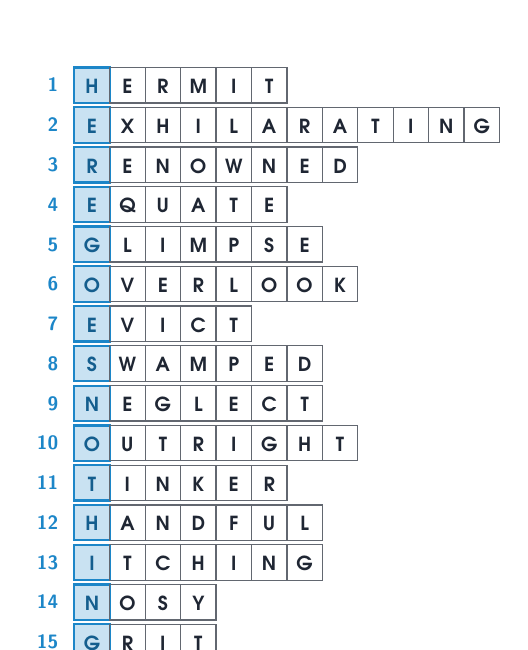
\begin{tikzpicture}[x=1mm,y=-1mm]
\node[anchor=east,font=\uifont\bfseries\scriptsize,text=accent] at (4.2,2.25) {1};
\fill[accent!24] (5.00,0.00) rectangle +(4.5,4.5);
\draw[accent,line width=0.8pt] (5.00,0.00) rectangle +(4.5,4.5);
\node[font=\hfont\bfseries\scriptsize,text=accentdark] at (7.25,2.40) {H};
\draw[ink!70,line width=0.45pt] (9.50,0.00) rectangle +(4.5,4.5);
\node[font=\hfont\bfseries\scriptsize,text=ink] at (11.75,2.40) {E};
\draw[ink!70,line width=0.45pt] (14.00,0.00) rectangle +(4.5,4.5);
\node[font=\hfont\bfseries\scriptsize,text=ink] at (16.25,2.40) {R};
\draw[ink!70,line width=0.45pt] (18.50,0.00) rectangle +(4.5,4.5);
\node[font=\hfont\bfseries\scriptsize,text=ink] at (20.75,2.40) {M};
\draw[ink!70,line width=0.45pt] (23.00,0.00) rectangle +(4.5,4.5);
\node[font=\hfont\bfseries\scriptsize,text=ink] at (25.25,2.40) {I};
\draw[ink!70,line width=0.45pt] (27.50,0.00) rectangle +(4.5,4.5);
\node[font=\hfont\bfseries\scriptsize,text=ink] at (29.75,2.40) {T};
\node[anchor=east,font=\uifont\bfseries\scriptsize,text=accent] at (4.2,7.30) {2};
\fill[accent!24] (5.00,5.05) rectangle +(4.5,4.5);
\draw[accent,line width=0.8pt] (5.00,5.05) rectangle +(4.5,4.5);
\node[font=\hfont\bfseries\scriptsize,text=accentdark] at (7.25,7.45) {E};
\draw[ink!70,line width=0.45pt] (9.50,5.05) rectangle +(4.5,4.5);
\node[font=\hfont\bfseries\scriptsize,text=ink] at (11.75,7.45) {X};
\draw[ink!70,line width=0.45pt] (14.00,5.05) rectangle +(4.5,4.5);
\node[font=\hfont\bfseries\scriptsize,text=ink] at (16.25,7.45) {H};
\draw[ink!70,line width=0.45pt] (18.50,5.05) rectangle +(4.5,4.5);
\node[font=\hfont\bfseries\scriptsize,text=ink] at (20.75,7.45) {I};
\draw[ink!70,line width=0.45pt] (23.00,5.05) rectangle +(4.5,4.5);
\node[font=\hfont\bfseries\scriptsize,text=ink] at (25.25,7.45) {L};
\draw[ink!70,line width=0.45pt] (27.50,5.05) rectangle +(4.5,4.5);
\node[font=\hfont\bfseries\scriptsize,text=ink] at (29.75,7.45) {A};
\draw[ink!70,line width=0.45pt] (32.00,5.05) rectangle +(4.5,4.5);
\node[font=\hfont\bfseries\scriptsize,text=ink] at (34.25,7.45) {R};
\draw[ink!70,line width=0.45pt] (36.50,5.05) rectangle +(4.5,4.5);
\node[font=\hfont\bfseries\scriptsize,text=ink] at (38.75,7.45) {A};
\draw[ink!70,line width=0.45pt] (41.00,5.05) rectangle +(4.5,4.5);
\node[font=\hfont\bfseries\scriptsize,text=ink] at (43.25,7.45) {T};
\draw[ink!70,line width=0.45pt] (45.50,5.05) rectangle +(4.5,4.5);
\node[font=\hfont\bfseries\scriptsize,text=ink] at (47.75,7.45) {I};
\draw[ink!70,line width=0.45pt] (50.00,5.05) rectangle +(4.5,4.5);
\node[font=\hfont\bfseries\scriptsize,text=ink] at (52.25,7.45) {N};
\draw[ink!70,line width=0.45pt] (54.50,5.05) rectangle +(4.5,4.5);
\node[font=\hfont\bfseries\scriptsize,text=ink] at (56.75,7.45) {G};
\node[anchor=east,font=\uifont\bfseries\scriptsize,text=accent] at (4.2,12.35) {3};
\fill[accent!24] (5.00,10.10) rectangle +(4.5,4.5);
\draw[accent,line width=0.8pt] (5.00,10.10) rectangle +(4.5,4.5);
\node[font=\hfont\bfseries\scriptsize,text=accentdark] at (7.25,12.50) {R};
\draw[ink!70,line width=0.45pt] (9.50,10.10) rectangle +(4.5,4.5);
\node[font=\hfont\bfseries\scriptsize,text=ink] at (11.75,12.50) {E};
\draw[ink!70,line width=0.45pt] (14.00,10.10) rectangle +(4.5,4.5);
\node[font=\hfont\bfseries\scriptsize,text=ink] at (16.25,12.50) {N};
\draw[ink!70,line width=0.45pt] (18.50,10.10) rectangle +(4.5,4.5);
\node[font=\hfont\bfseries\scriptsize,text=ink] at (20.75,12.50) {O};
\draw[ink!70,line width=0.45pt] (23.00,10.10) rectangle +(4.5,4.5);
\node[font=\hfont\bfseries\scriptsize,text=ink] at (25.25,12.50) {W};
\draw[ink!70,line width=0.45pt] (27.50,10.10) rectangle +(4.5,4.5);
\node[font=\hfont\bfseries\scriptsize,text=ink] at (29.75,12.50) {N};
\draw[ink!70,line width=0.45pt] (32.00,10.10) rectangle +(4.5,4.5);
\node[font=\hfont\bfseries\scriptsize,text=ink] at (34.25,12.50) {E};
\draw[ink!70,line width=0.45pt] (36.50,10.10) rectangle +(4.5,4.5);
\node[font=\hfont\bfseries\scriptsize,text=ink] at (38.75,12.50) {D};
\node[anchor=east,font=\uifont\bfseries\scriptsize,text=accent] at (4.2,17.40) {4};
\fill[accent!24] (5.00,15.15) rectangle +(4.5,4.5);
\draw[accent,line width=0.8pt] (5.00,15.15) rectangle +(4.5,4.5);
\node[font=\hfont\bfseries\scriptsize,text=accentdark] at (7.25,17.55) {E};
\draw[ink!70,line width=0.45pt] (9.50,15.15) rectangle +(4.5,4.5);
\node[font=\hfont\bfseries\scriptsize,text=ink] at (11.75,17.55) {Q};
\draw[ink!70,line width=0.45pt] (14.00,15.15) rectangle +(4.5,4.5);
\node[font=\hfont\bfseries\scriptsize,text=ink] at (16.25,17.55) {U};
\draw[ink!70,line width=0.45pt] (18.50,15.15) rectangle +(4.5,4.5);
\node[font=\hfont\bfseries\scriptsize,text=ink] at (20.75,17.55) {A};
\draw[ink!70,line width=0.45pt] (23.00,15.15) rectangle +(4.5,4.5);
\node[font=\hfont\bfseries\scriptsize,text=ink] at (25.25,17.55) {T};
\draw[ink!70,line width=0.45pt] (27.50,15.15) rectangle +(4.5,4.5);
\node[font=\hfont\bfseries\scriptsize,text=ink] at (29.75,17.55) {E};
\node[anchor=east,font=\uifont\bfseries\scriptsize,text=accent] at (4.2,22.45) {5};
\fill[accent!24] (5.00,20.20) rectangle +(4.5,4.5);
\draw[accent,line width=0.8pt] (5.00,20.20) rectangle +(4.5,4.5);
\node[font=\hfont\bfseries\scriptsize,text=accentdark] at (7.25,22.60) {G};
\draw[ink!70,line width=0.45pt] (9.50,20.20) rectangle +(4.5,4.5);
\node[font=\hfont\bfseries\scriptsize,text=ink] at (11.75,22.60) {L};
\draw[ink!70,line width=0.45pt] (14.00,20.20) rectangle +(4.5,4.5);
\node[font=\hfont\bfseries\scriptsize,text=ink] at (16.25,22.60) {I};
\draw[ink!70,line width=0.45pt] (18.50,20.20) rectangle +(4.5,4.5);
\node[font=\hfont\bfseries\scriptsize,text=ink] at (20.75,22.60) {M};
\draw[ink!70,line width=0.45pt] (23.00,20.20) rectangle +(4.5,4.5);
\node[font=\hfont\bfseries\scriptsize,text=ink] at (25.25,22.60) {P};
\draw[ink!70,line width=0.45pt] (27.50,20.20) rectangle +(4.5,4.5);
\node[font=\hfont\bfseries\scriptsize,text=ink] at (29.75,22.60) {S};
\draw[ink!70,line width=0.45pt] (32.00,20.20) rectangle +(4.5,4.5);
\node[font=\hfont\bfseries\scriptsize,text=ink] at (34.25,22.60) {E};
\node[anchor=east,font=\uifont\bfseries\scriptsize,text=accent] at (4.2,27.50) {6};
\fill[accent!24] (5.00,25.25) rectangle +(4.5,4.5);
\draw[accent,line width=0.8pt] (5.00,25.25) rectangle +(4.5,4.5);
\node[font=\hfont\bfseries\scriptsize,text=accentdark] at (7.25,27.65) {O};
\draw[ink!70,line width=0.45pt] (9.50,25.25) rectangle +(4.5,4.5);
\node[font=\hfont\bfseries\scriptsize,text=ink] at (11.75,27.65) {V};
\draw[ink!70,line width=0.45pt] (14.00,25.25) rectangle +(4.5,4.5);
\node[font=\hfont\bfseries\scriptsize,text=ink] at (16.25,27.65) {E};
\draw[ink!70,line width=0.45pt] (18.50,25.25) rectangle +(4.5,4.5);
\node[font=\hfont\bfseries\scriptsize,text=ink] at (20.75,27.65) {R};
\draw[ink!70,line width=0.45pt] (23.00,25.25) rectangle +(4.5,4.5);
\node[font=\hfont\bfseries\scriptsize,text=ink] at (25.25,27.65) {L};
\draw[ink!70,line width=0.45pt] (27.50,25.25) rectangle +(4.5,4.5);
\node[font=\hfont\bfseries\scriptsize,text=ink] at (29.75,27.65) {O};
\draw[ink!70,line width=0.45pt] (32.00,25.25) rectangle +(4.5,4.5);
\node[font=\hfont\bfseries\scriptsize,text=ink] at (34.25,27.65) {O};
\draw[ink!70,line width=0.45pt] (36.50,25.25) rectangle +(4.5,4.5);
\node[font=\hfont\bfseries\scriptsize,text=ink] at (38.75,27.65) {K};
\node[anchor=east,font=\uifont\bfseries\scriptsize,text=accent] at (4.2,32.55) {7};
\fill[accent!24] (5.00,30.30) rectangle +(4.5,4.5);
\draw[accent,line width=0.8pt] (5.00,30.30) rectangle +(4.5,4.5);
\node[font=\hfont\bfseries\scriptsize,text=accentdark] at (7.25,32.70) {E};
\draw[ink!70,line width=0.45pt] (9.50,30.30) rectangle +(4.5,4.5);
\node[font=\hfont\bfseries\scriptsize,text=ink] at (11.75,32.70) {V};
\draw[ink!70,line width=0.45pt] (14.00,30.30) rectangle +(4.5,4.5);
\node[font=\hfont\bfseries\scriptsize,text=ink] at (16.25,32.70) {I};
\draw[ink!70,line width=0.45pt] (18.50,30.30) rectangle +(4.5,4.5);
\node[font=\hfont\bfseries\scriptsize,text=ink] at (20.75,32.70) {C};
\draw[ink!70,line width=0.45pt] (23.00,30.30) rectangle +(4.5,4.5);
\node[font=\hfont\bfseries\scriptsize,text=ink] at (25.25,32.70) {T};
\node[anchor=east,font=\uifont\bfseries\scriptsize,text=accent] at (4.2,37.60) {8};
\fill[accent!24] (5.00,35.35) rectangle +(4.5,4.5);
\draw[accent,line width=0.8pt] (5.00,35.35) rectangle +(4.5,4.5);
\node[font=\hfont\bfseries\scriptsize,text=accentdark] at (7.25,37.75) {S};
\draw[ink!70,line width=0.45pt] (9.50,35.35) rectangle +(4.5,4.5);
\node[font=\hfont\bfseries\scriptsize,text=ink] at (11.75,37.75) {W};
\draw[ink!70,line width=0.45pt] (14.00,35.35) rectangle +(4.5,4.5);
\node[font=\hfont\bfseries\scriptsize,text=ink] at (16.25,37.75) {A};
\draw[ink!70,line width=0.45pt] (18.50,35.35) rectangle +(4.5,4.5);
\node[font=\hfont\bfseries\scriptsize,text=ink] at (20.75,37.75) {M};
\draw[ink!70,line width=0.45pt] (23.00,35.35) rectangle +(4.5,4.5);
\node[font=\hfont\bfseries\scriptsize,text=ink] at (25.25,37.75) {P};
\draw[ink!70,line width=0.45pt] (27.50,35.35) rectangle +(4.5,4.5);
\node[font=\hfont\bfseries\scriptsize,text=ink] at (29.75,37.75) {E};
\draw[ink!70,line width=0.45pt] (32.00,35.35) rectangle +(4.5,4.5);
\node[font=\hfont\bfseries\scriptsize,text=ink] at (34.25,37.75) {D};
\node[anchor=east,font=\uifont\bfseries\scriptsize,text=accent] at (4.2,42.65) {9};
\fill[accent!24] (5.00,40.40) rectangle +(4.5,4.5);
\draw[accent,line width=0.8pt] (5.00,40.40) rectangle +(4.5,4.5);
\node[font=\hfont\bfseries\scriptsize,text=accentdark] at (7.25,42.80) {N};
\draw[ink!70,line width=0.45pt] (9.50,40.40) rectangle +(4.5,4.5);
\node[font=\hfont\bfseries\scriptsize,text=ink] at (11.75,42.80) {E};
\draw[ink!70,line width=0.45pt] (14.00,40.40) rectangle +(4.5,4.5);
\node[font=\hfont\bfseries\scriptsize,text=ink] at (16.25,42.80) {G};
\draw[ink!70,line width=0.45pt] (18.50,40.40) rectangle +(4.5,4.5);
\node[font=\hfont\bfseries\scriptsize,text=ink] at (20.75,42.80) {L};
\draw[ink!70,line width=0.45pt] (23.00,40.40) rectangle +(4.5,4.5);
\node[font=\hfont\bfseries\scriptsize,text=ink] at (25.25,42.80) {E};
\draw[ink!70,line width=0.45pt] (27.50,40.40) rectangle +(4.5,4.5);
\node[font=\hfont\bfseries\scriptsize,text=ink] at (29.75,42.80) {C};
\draw[ink!70,line width=0.45pt] (32.00,40.40) rectangle +(4.5,4.5);
\node[font=\hfont\bfseries\scriptsize,text=ink] at (34.25,42.80) {T};
\node[anchor=east,font=\uifont\bfseries\scriptsize,text=accent] at (4.2,47.70) {10};
\fill[accent!24] (5.00,45.45) rectangle +(4.5,4.5);
\draw[accent,line width=0.8pt] (5.00,45.45) rectangle +(4.5,4.5);
\node[font=\hfont\bfseries\scriptsize,text=accentdark] at (7.25,47.85) {O};
\draw[ink!70,line width=0.45pt] (9.50,45.45) rectangle +(4.5,4.5);
\node[font=\hfont\bfseries\scriptsize,text=ink] at (11.75,47.85) {U};
\draw[ink!70,line width=0.45pt] (14.00,45.45) rectangle +(4.5,4.5);
\node[font=\hfont\bfseries\scriptsize,text=ink] at (16.25,47.85) {T};
\draw[ink!70,line width=0.45pt] (18.50,45.45) rectangle +(4.5,4.5);
\node[font=\hfont\bfseries\scriptsize,text=ink] at (20.75,47.85) {R};
\draw[ink!70,line width=0.45pt] (23.00,45.45) rectangle +(4.5,4.5);
\node[font=\hfont\bfseries\scriptsize,text=ink] at (25.25,47.85) {I};
\draw[ink!70,line width=0.45pt] (27.50,45.45) rectangle +(4.5,4.5);
\node[font=\hfont\bfseries\scriptsize,text=ink] at (29.75,47.85) {G};
\draw[ink!70,line width=0.45pt] (32.00,45.45) rectangle +(4.5,4.5);
\node[font=\hfont\bfseries\scriptsize,text=ink] at (34.25,47.85) {H};
\draw[ink!70,line width=0.45pt] (36.50,45.45) rectangle +(4.5,4.5);
\node[font=\hfont\bfseries\scriptsize,text=ink] at (38.75,47.85) {T};
\node[anchor=east,font=\uifont\bfseries\scriptsize,text=accent] at (4.2,52.75) {11};
\fill[accent!24] (5.00,50.50) rectangle +(4.5,4.5);
\draw[accent,line width=0.8pt] (5.00,50.50) rectangle +(4.5,4.5);
\node[font=\hfont\bfseries\scriptsize,text=accentdark] at (7.25,52.90) {T};
\draw[ink!70,line width=0.45pt] (9.50,50.50) rectangle +(4.5,4.5);
\node[font=\hfont\bfseries\scriptsize,text=ink] at (11.75,52.90) {I};
\draw[ink!70,line width=0.45pt] (14.00,50.50) rectangle +(4.5,4.5);
\node[font=\hfont\bfseries\scriptsize,text=ink] at (16.25,52.90) {N};
\draw[ink!70,line width=0.45pt] (18.50,50.50) rectangle +(4.5,4.5);
\node[font=\hfont\bfseries\scriptsize,text=ink] at (20.75,52.90) {K};
\draw[ink!70,line width=0.45pt] (23.00,50.50) rectangle +(4.5,4.5);
\node[font=\hfont\bfseries\scriptsize,text=ink] at (25.25,52.90) {E};
\draw[ink!70,line width=0.45pt] (27.50,50.50) rectangle +(4.5,4.5);
\node[font=\hfont\bfseries\scriptsize,text=ink] at (29.75,52.90) {R};
\node[anchor=east,font=\uifont\bfseries\scriptsize,text=accent] at (4.2,57.80) {12};
\fill[accent!24] (5.00,55.55) rectangle +(4.5,4.5);
\draw[accent,line width=0.8pt] (5.00,55.55) rectangle +(4.5,4.5);
\node[font=\hfont\bfseries\scriptsize,text=accentdark] at (7.25,57.95) {H};
\draw[ink!70,line width=0.45pt] (9.50,55.55) rectangle +(4.5,4.5);
\node[font=\hfont\bfseries\scriptsize,text=ink] at (11.75,57.95) {A};
\draw[ink!70,line width=0.45pt] (14.00,55.55) rectangle +(4.5,4.5);
\node[font=\hfont\bfseries\scriptsize,text=ink] at (16.25,57.95) {N};
\draw[ink!70,line width=0.45pt] (18.50,55.55) rectangle +(4.5,4.5);
\node[font=\hfont\bfseries\scriptsize,text=ink] at (20.75,57.95) {D};
\draw[ink!70,line width=0.45pt] (23.00,55.55) rectangle +(4.5,4.5);
\node[font=\hfont\bfseries\scriptsize,text=ink] at (25.25,57.95) {F};
\draw[ink!70,line width=0.45pt] (27.50,55.55) rectangle +(4.5,4.5);
\node[font=\hfont\bfseries\scriptsize,text=ink] at (29.75,57.95) {U};
\draw[ink!70,line width=0.45pt] (32.00,55.55) rectangle +(4.5,4.5);
\node[font=\hfont\bfseries\scriptsize,text=ink] at (34.25,57.95) {L};
\node[anchor=east,font=\uifont\bfseries\scriptsize,text=accent] at (4.2,62.85) {13};
\fill[accent!24] (5.00,60.60) rectangle +(4.5,4.5);
\draw[accent,line width=0.8pt] (5.00,60.60) rectangle +(4.5,4.5);
\node[font=\hfont\bfseries\scriptsize,text=accentdark] at (7.25,63.00) {I};
\draw[ink!70,line width=0.45pt] (9.50,60.60) rectangle +(4.5,4.5);
\node[font=\hfont\bfseries\scriptsize,text=ink] at (11.75,63.00) {T};
\draw[ink!70,line width=0.45pt] (14.00,60.60) rectangle +(4.5,4.5);
\node[font=\hfont\bfseries\scriptsize,text=ink] at (16.25,63.00) {C};
\draw[ink!70,line width=0.45pt] (18.50,60.60) rectangle +(4.5,4.5);
\node[font=\hfont\bfseries\scriptsize,text=ink] at (20.75,63.00) {H};
\draw[ink!70,line width=0.45pt] (23.00,60.60) rectangle +(4.5,4.5);
\node[font=\hfont\bfseries\scriptsize,text=ink] at (25.25,63.00) {I};
\draw[ink!70,line width=0.45pt] (27.50,60.60) rectangle +(4.5,4.5);
\node[font=\hfont\bfseries\scriptsize,text=ink] at (29.75,63.00) {N};
\draw[ink!70,line width=0.45pt] (32.00,60.60) rectangle +(4.5,4.5);
\node[font=\hfont\bfseries\scriptsize,text=ink] at (34.25,63.00) {G};
\node[anchor=east,font=\uifont\bfseries\scriptsize,text=accent] at (4.2,67.90) {14};
\fill[accent!24] (5.00,65.65) rectangle +(4.5,4.5);
\draw[accent,line width=0.8pt] (5.00,65.65) rectangle +(4.5,4.5);
\node[font=\hfont\bfseries\scriptsize,text=accentdark] at (7.25,68.05) {N};
\draw[ink!70,line width=0.45pt] (9.50,65.65) rectangle +(4.5,4.5);
\node[font=\hfont\bfseries\scriptsize,text=ink] at (11.75,68.05) {O};
\draw[ink!70,line width=0.45pt] (14.00,65.65) rectangle +(4.5,4.5);
\node[font=\hfont\bfseries\scriptsize,text=ink] at (16.25,68.05) {S};
\draw[ink!70,line width=0.45pt] (18.50,65.65) rectangle +(4.5,4.5);
\node[font=\hfont\bfseries\scriptsize,text=ink] at (20.75,68.05) {Y};
\node[anchor=east,font=\uifont\bfseries\scriptsize,text=accent] at (4.2,72.95) {15};
\fill[accent!24] (5.00,70.70) rectangle +(4.5,4.5);
\draw[accent,line width=0.8pt] (5.00,70.70) rectangle +(4.5,4.5);
\node[font=\hfont\bfseries\scriptsize,text=accentdark] at (7.25,73.10) {G};
\draw[ink!70,line width=0.45pt] (9.50,70.70) rectangle +(4.5,4.5);
\node[font=\hfont\bfseries\scriptsize,text=ink] at (11.75,73.10) {R};
\draw[ink!70,line width=0.45pt] (14.00,70.70) rectangle +(4.5,4.5);
\node[font=\hfont\bfseries\scriptsize,text=ink] at (16.25,73.10) {I};
\draw[ink!70,line width=0.45pt] (18.50,70.70) rectangle +(4.5,4.5);
\node[font=\hfont\bfseries\scriptsize,text=ink] at (20.75,73.10) {T};
\end{tikzpicture}
\end{minipage}\hfill
\begin{minipage}[t]{0.6\linewidth}\vspace{0pt}\small\RaggedRight
\setlength{\parskip}{1.2pt}
\num{1} \textbf{hermit} \mMT\,{\uifont\fontsize{5.4}{6}\selectfont\color{mute}OCT} \quad \num{2} \textbf{exhilarating} \mDS\,{\uifont\fontsize{5.4}{6}\selectfont\color{mute}OCT}\par
\num{3} \textbf{renowned} \mDBZ\,{\uifont\fontsize{5.4}{6}\selectfont\color{mute}MAR} \quad \num{4} \textbf{equate} \mDBZ\,{\uifont\fontsize{5.4}{6}\selectfont\color{mute}MAR}\par
\num{5} \textbf{glimpse} \mJJK\,{\uifont\fontsize{5.4}{6}\selectfont\color{mute}MAR} \quad \num{6} \textbf{overlook} \mMHA\,{\uifont\fontsize{5.4}{6}\selectfont\color{mute}MAR}\par
\num{7} \textbf{evict} \mMHA\,{\uifont\fontsize{5.4}{6}\selectfont\color{mute}MAR} \quad \num{8} \textbf{swamped} \mMHA\,{\uifont\fontsize{5.4}{6}\selectfont\color{mute}MAR}\par
\num{9} \textbf{neglect} \mJJK\,{\uifont\fontsize{5.4}{6}\selectfont\color{mute}MAR} \quad \num{10} \textbf{outright} \mJJK\,{\uifont\fontsize{5.4}{6}\selectfont\color{mute}MAR}\par
\num{11} \textbf{tinker} \mJJK\,{\uifont\fontsize{5.4}{6}\selectfont\color{mute}MAR} \quad \num{12} \textbf{handful} \mDBZ\,{\uifont\fontsize{5.4}{6}\selectfont\color{mute}MAR}\par
\num{13} \textbf{itching} \mDBZ\,{\uifont\fontsize{5.4}{6}\selectfont\color{mute}MAR} \quad \num{14} \textbf{nosy} {\color{inksoft}/ nosey} \mMHA\,{\uifont\fontsize{5.4}{6}\selectfont\color{mute}MAR}\par
\num{15} \textbf{grit} \mLF\,{\uifont\fontsize{5.4}{6}\selectfont\color{mute}OCT}\par\vspace{2mm}
\textbf{The phrase: HERE GOES NOTHING} \mDBZ\,{\uifont\fontsize{5.4}{6}\selectfont\color{mute}MAR} — what you say just before you try something risky that may well fail: \emph{“Right… here goes nothing.”}\par\vspace{2mm}
\why{Spelling traps (tag \tgA{F}): ex\textbf{h}ilarating keeps the silent \emph{h} and has one \emph{l}; \emph{renowned} has no \emph{k} (it is not from \emph{known}); \emph{tinker \textbf{with}} something. If the meaning was right but the spelling wrong, tag it F, not M.}
\end{minipage}

% ===================================================================== PART 2
\akhead{4}{One word, three jobs}{\tgA{S}}
\begin{multicols}{2}
\begin{aitem}\ai{1}{\textbf{keen}}{\mDBZ\,{\uifont\fontsize{5.4}{6}\selectfont\color{mute}MAR}}\an{\lab{a} \emph{keen on} = enthusiastic about (\UK{} favourite) \mdot{} \lab{b} a \emph{keen eye} = sharp perception \mdot{} \lab{c} a \emph{keen edge} = a sharp blade.}\end{aitem}
\begin{aitem}\ai{2}{\textbf{coast}}{\mDBZ\,{\uifont\fontsize{5.4}{6}\selectfont\color{mute}MAR}}\an{\lab{a} the seashore \mdot{} \lab{b} \emph{coasted through} = succeeded with little effort \mdot{} \lab{c} \emph{coasted} = moved without power.}\end{aitem}
\begin{aitem}\ai{3}{\textbf{floor}}{\mDBZ\,{\uifont\fontsize{5.4}{6}\selectfont\color{mute}MAR}}\an{\lab{a} a level of a building \mdot{} \lab{b} \emph{floored} = shocked, left speechless \mdot{} \lab{c} \emph{give someone the floor} = the right to speak. \UK{} the \emph{ground floor} is the American \emph{first floor}.}\end{aitem}
\begin{aitem}\ai{4}{\textbf{sheer}}{\mJJK\,{\uifont\fontsize{5.4}{6}\selectfont\color{mute}MAR}}\an{\lab{a} \emph{sheer luck} = pure, nothing but \mdot{} \lab{b} \emph{a sheer drop} = almost vertical \mdot{} \lab{c} \emph{sheer fabric} = thin and see-through.}\end{aitem}
\begin{aitem}\ai{5}{\textbf{toll}}{\mJJK\,{\uifont\fontsize{5.4}{6}\selectfont\color{mute}MAR}}\an{\lab{a} \emph{death toll} = number of deaths \mdot{} \lab{b} a fee to use a road \mdot{} \lab{c} bells \emph{toll} = ring slowly. \newsense{} \emph{take its toll (on)}: \emph{Night shifts took their toll on his health.}}\end{aitem}
\begin{aitem}\ai{6}{\textbf{stem}}{\mJJK\,{\uifont\fontsize{5.4}{6}\selectfont\color{mute}MAR}}\an{\lab{a} \emph{stem from} = come from, be caused by \mdot{} \lab{b} \emph{stem the flow} = stop it \mdot{} \lab{c} the stalk of a flower.}\end{aitem}
\begin{aitem}\ai{7}{\textbf{surge}}{\mJJK\,{\uifont\fontsize{5.4}{6}\selectfont\color{mute}FEB}}\an{\lab{a} a sudden big increase \mdot{} \lab{b} a sudden strong feeling \mdot{} \lab{c} \emph{a power surge}. (\emph{Spike} fits a and c, but not \emph{a spike of panic}.)}\end{aitem}
\begin{aitem}\ai{8}{\textbf{hail}}{\mDBS\,{\uifont\fontsize{5.4}{6}\selectfont\color{mute}OCT}}\an{\lab{a} \emph{hailed as} = publicly praised as (headline favourite) \mdot{} \lab{b} wave to stop a taxi \mdot{} \lab{c} balls of ice. Bonus sense: \emph{he hails from Porto} = comes from.}\end{aitem}
\begin{aitem}\ai{9}{\textbf{lodge}}{\mDBZ\,{\uifont\fontsize{5.4}{6}\selectfont\color{mute}OCT}}\an{\lab{a} \emph{lodged} = firmly stuck \mdot{} \lab{b} \emph{lodge a complaint} = make it officially \mdot{} \lab{c} a small house in the mountains.}\end{aitem}
\begin{aitem}\ai{10}{\textbf{strain}}{\mDBZ\,{\uifont\fontsize{5.4}{6}\selectfont\color{mute}JAN}}\an{\lab{a} pressure, stress \mdot{} \lab{b} \emph{strained} = injured by over-stretching \mdot{} \lab{c} pour through a sieve. Bonus: \emph{a new strain of the virus}.}\end{aitem}
\end{multicols}

\akhead{5}{Volume knobs}{\tgA{N}}
\begin{multicols}{2}
\begin{aitem}\ai{}{{\hfont\footnotesize EFFORT}: \textbf{slack off \arr{} coast \arr{} buckle down \arr{} work your tail off}}{}\an{Slacking off = deliberately doing less than you should; coasting = cruising on minimum effort (often still passing); buckling down = getting serious.}\end{aitem}
\begin{aitem}\ai{}{{\hfont\footnotesize RESISTANCE}: \textbf{hesitant \arr{} reluctant \arr{} balk at \arr{} defiant}}{}\an{Hesitant = unsure, pausing; reluctant = unwilling but may still do it; balk at = refuse to go on (like a horse at a fence); defiant = openly refusing, challenging.}\end{aitem}
\begin{aitem}\ai{}{{\hfont\footnotesize TROUBLE}: \textbf{snag \arr{} ordeal \arr{} calamity}}{}\end{aitem}
\begin{aitem}\ai{}{{\hfont\footnotesize CONFLICT}: \textbf{bickering \arr{} quarrel \arr{} onslaught}}{}\an{Bickering is petty; an onslaught is a violent attack (or a flood of criticism).}\end{aitem}
\begin{aitem}\ai{}{{\hfont\footnotesize LAUGHTER}: \textbf{grin \arr{} giggle \arr{} crack up}}{}\end{aitem}
\begin{aitem}\ai{}{{\hfont\footnotesize NERVE}: \textbf{sassy \arr{} impudent \arr{} brazen}}{}\an{Sass is cheeky and often playful; impudent is rude; brazen is shameless.}\end{aitem}
\end{multicols}
\model{\textbf{Turn it up — model:} \emph{I worked my tail off all week, so when my housemate offered a brazen excuse for not doing the washing-up again, I just cracked up.}}

\akhead{6}{Mic check}{\tgA{F}\,\tgA{B}}
\sub{A \enspace Homophones \enspace\tgA{F}}
{\small \num{1} \textbf{tail} \mDS\,{\uifont\fontsize{5.4}{6}\selectfont\color{mute}OCT} \enspace \num{2} \textbf{fare} \mDBZ\,{\uifont\fontsize{5.4}{6}\selectfont\color{mute}MAR} \enspace \num{3} \textbf{feat} \mDBZ\,{\uifont\fontsize{5.4}{6}\selectfont\color{mute}MAR} \enspace \num{4} \textbf{meddling} \mDBZ\,{\uifont\fontsize{5.4}{6}\selectfont\color{mute}JAN} \enspace \num{5} \textbf{reek} \mDS\,{\uifont\fontsize{5.4}{6}\selectfont\color{mute}OCT} \enspace \num{6} \textbf{sole} \mJJK\,{\uifont\fontsize{5.4}{6}\selectfont\color{mute}MAR} \enspace \num{7} \textbf{flour} \mJJK\,{\uifont\fontsize{5.4}{6}\selectfont\color{mute}MAR} \enspace \num{8} \textbf{long-haul} \mDS\,{\uifont\fontsize{5.4}{6}\selectfont\color{mute}OCT}}
\sub{B \enspace Silent letters \enspace\tgA{F}}
{\small\begin{multicols}{2}\RaggedRight
subtle — \textbf{b} \enspace\ipa{/"s2tl/}\par
heirloom — \textbf{h} \enspace\ipa{/"e@lu:m/}\par
numb — \textbf{b} \enspace\ipa{/n2m/}\par
knack — \textbf{k} \enspace\ipa{/n\ae k/}\par
wrestling — \textbf{w}, \textbf{t} \enspace\ipa{/"reslIN/}\par
wrath — \textbf{w} \enspace\ipa{/r6T/} \enspace{\footnotesize\color{inksoft}(US \ipa{/r\ae T/})}\par
reigning — \textbf{g} \enspace\ipa{/"reInIN/}\par
psyche — \textbf{p} \enspace\ipa{/"saIki/}\par
doughy — \textbf{gh} \enspace\ipa{/"d@Ui/}\par
listen up — \textbf{t} \enspace\ipa{/"lIsn/}\par
\end{multicols}}
\sub{C \enspace The British \ipa{/A:/} \enspace\tgA{B}}
{\small \textbf{grasp, chant, slander, rascal, half-pint, laughingstock} have \ipa{/A:/} in standard southern British English (\ipa{/grA:sp/, /tSA:nt/}). \emph{Ample, anvil, dashing, scram, racket, tandem} keep the short \ipa{/\ae/} everywhere.}
\an{Ear training for voice chat: speakers from the north of England use the short vowel in all twelve — \emph{grass} and \emph{gas} have the same vowel there. So both pronunciations are British; the long one is the southern standard.}
\sub{D \enspace Stress \enspace\tgA{F}}
{\small\begin{multicols}{2}\RaggedRight
un\textbf{\underline{PRE}}cedented \enspace\ipa{/2n"presIdentId/}\par
om\textbf{\underline{NI}}scient \enspace\ipa{/6m"nIsi@nt/}\par
ex\textbf{\underline{EM}}plary \enspace\ipa{/Ig"zempl@ri/}\par
ca\textbf{\underline{LA}}mity \enspace\ipa{/k@"l\ae m@ti/}\par
sab\textbf{\underline{BA}}tical \enspace\ipa{/s@"b\ae tIkl/}\par
con\textbf{\underline{TIN}}gency \enspace\ipa{/k@n"tIndZ@nsi/}\par
\textbf{\underline{BU}}reaucrat \enspace\ipa{/"bjU@r@kr\ae t/}\par
vo\textbf{\underline{CI}}ferously \enspace\ipa{/v@"sIf@r@sli/}\par
\textbf{\underline{CON}}voluted \enspace\ipa{/"k6nv@lu:tId/}\par
\textbf{\underline{LE}}niency \enspace\ipa{/"li:ni@nsi/}\par
\end{multicols}}

% ===================================================================== PART 3
\akhead{7}{Compliment or insult?}{\tgA{N}\,\tgA{R}}
{\small\noindent\textbf{C — compliments:} shrewd, resourceful, nimble, exemplary, feisty, laid-back, dashing.\par
\noindent\textbf{I — insults:} gullible, stuck-up, nosy, cocky, smooth-talking, pigheaded, obnoxious.\par
\noindent\textbf{D — it depends:} cunning, scrappy, naive, defiant, mischievous, portly.}
\an{\emph{Cunning}: admiring for a clever move in a game, negative about someone’s character. \emph{Scrappy} \mMHA\,{\uifont\fontsize{5.4}{6}\selectfont\color{mute}MAR}: in American English a small, determined fighter (praise); in British English \emph{a scrappy match / scrappy notes} = messy, disorganised \newsense. \emph{Naive}: inexperienced — gentle criticism, not an insult. \emph{Defiant}: brave resistance or plain disobedience. \emph{Mischievous}: playful or harmful. \emph{Portly}: an old-fashioned, polite word for fat — gentle word, sensitive topic. \emph{Feisty} is praise, but some people find it patronising when it is said about women.}
\model{\textbf{Flip it — model (cunning):} \emph{That was a cunning move — you baited their whole team into the corner.} / \emph{Don’t trust him; he’s cunning and he only looks after himself.}}

\akhead{8}{Not quite twins}{\tgA{N}\,\tgA{C}}
\sub{A \enspace Stopping things}
{\small\noindent\textbf{hinder} \ding{172} \enspace \textbf{impede} \ding{172}\,\ding{177} \enspace \textbf{thwart} \ding{173} \enspace \textbf{foil} \ding{173} \enspace \textbf{ward off} \ding{174} \enspace \textbf{fend off} \ding{174}\,\ding{175} \enspace \textbf{hold off} \ding{174}\,\ding{176}}
\begin{multicols}{2}
\begin{aitem}\ai{a}{\textbf{foiled} / {\color{inksoft}thwarted}}{\mDBZ\,{\uifont\fontsize{5.4}{6}\selectfont\color{mute}MAR}}\an{\emph{Foil} is the classic newspaper verb for plots and crimes; \emph{thwart} is broader (\emph{thwart someone’s plans}).}\end{aitem}
\begin{aitem}\ai{b}{\textbf{ward off}}{\mJJK\,{\uifont\fontsize{5.4}{6}\selectfont\color{mute}FEB}}\end{aitem}
\begin{aitem}\ai{c}{\textbf{hindered} / {\color{inksoft}impeded}}{\mMHA\,{\uifont\fontsize{5.4}{6}\selectfont\color{mute}MAR}}\end{aitem}
\begin{aitem}\ai{d}{\textbf{fended off}}{\mDBZ\,{\uifont\fontsize{5.4}{6}\selectfont\color{mute}OCT}}\an{Only \emph{fend off} naturally takes questions and criticism.}\end{aitem}
\begin{aitem}\ai{e}{\textbf{hold off} {\color{inksoft}(on)}}{\mDBZ\,{\uifont\fontsize{5.4}{6}\selectfont\color{mute}MAR}}\an{\emph{hold off (on) doing something} = postpone it.}\end{aitem}
\begin{aitem}\ai{f}{\textbf{impede} / {\color{inksoft}hinder}}{\mDBZ\,{\uifont\fontsize{5.4}{6}\selectfont\color{mute}MAR}}\an{Both work; \emph{impede} is the formal, report-friendly choice.}\end{aitem}
\end{multicols}
\sub{B \enspace Who works for whom?}
{\small\noindent\textbf{henchman} \ding{172} \enspace \textbf{sidekick} \ding{173} \enspace \textbf{crony} \ding{174} \enspace \textbf{lackey} \ding{175} \enspace \textbf{underling} \ding{176} \enspace \textbf{pawn} \ding{177}}
\an{Overlaps are real (a henchman is usually a lackey too), but these are the defining features.}
{\small\noindent \num{g} \textbf{cronies} \mDBZ\,{\uifont\fontsize{5.4}{6}\selectfont\color{mute}MAR} \enspace \num{h} \textbf{sidekick} \mDBZ\,{\uifont\fontsize{5.4}{6}\selectfont\color{mute}MAR} \enspace \num{i} \textbf{henchmen} \mDBZ\,{\uifont\fontsize{5.4}{6}\selectfont\color{mute}MAR} \enspace \num{j} \textbf{lackey} \mJJK\,{\uifont\fontsize{5.4}{6}\selectfont\color{mute}MAR} \enspace \num{k} \textbf{pawn} \mDBZ\,{\uifont\fontsize{5.4}{6}\selectfont\color{mute}MAR} \enspace \num{l} \textbf{underlings} \mDBS\,{\uifont\fontsize{5.4}{6}\selectfont\color{mute}OCT}}
\sub{C \enspace Pick the precise one}
\begin{multicols}{2}
\begin{aitem}\ai{m}{\textbf{innate}}{\mMT\,{\uifont\fontsize{5.4}{6}\selectfont\color{mute}OCT}}\an{Present from birth.}\end{aitem}
\begin{aitem}\ai{n}{\textbf{inherent}}{\mJJK\,{\uifont\fontsize{5.4}{6}\selectfont\color{mute}MAR}}\an{Built into the nature of a thing — risks, flaws, limits.}\end{aitem}
\begin{aitem}\ai{o}{\textbf{seldom}}{\mLF\,{\uifont\fontsize{5.4}{6}\selectfont\color{mute}OCT}}\an{Frequency: rarely.}\end{aitem}
\begin{aitem}\ai{p}{\textbf{scarcely}}{\mDBZ\,{\uifont\fontsize{5.4}{6}\selectfont\color{mute}MAR}}\an{Degree: hardly, almost not.}\end{aitem}
\begin{aitem}\ai{q}{\textbf{merely}}{\mJJK\,{\uifont\fontsize{5.4}{6}\selectfont\color{mute}MAR}}\an{Only — to make something sound small.}\end{aitem}
\begin{aitem}\ai{r}{\textbf{utmost}}{\mDBZ\,{\uifont\fontsize{5.4}{6}\selectfont\color{mute}JAN}}\an{\vfix{} Your \emph{upmost} card calls it a variant spelling of \emph{utmost} — standard English is \emph{of the utmost importance}.}\end{aitem}
\begin{aitem}\ai{s}{\textbf{ensure}}{\mDBZ\,{\uifont\fontsize{5.4}{6}\selectfont\color{mute}MAR}}\an{\emph{Assure someone that\ldots} = tell them confidently; \emph{ensure} = make certain; \emph{insure} = buy insurance.}\end{aitem}
\begin{aitem}\ai{t}{\textbf{whereabouts}}{\mJJK\,{\uifont\fontsize{5.4}{6}\selectfont\color{mute}MAR}}\end{aitem}
\end{multicols}

\akhead{9}{The odd one out}{\tgA{C}}
\begin{multicols}{2}\small\RaggedRight
\textbf{harbour} — \sout{a threat} \arr{} \emph{pose} a threat\par\vspace{1mm}
\textbf{impose} — \sout{a question} \arr{} \emph{pose / ask}\par\vspace{1mm}
\textbf{withhold} — \sout{a meeting} \arr{} \emph{hold}\par\vspace{1mm}
\textbf{evoke} — \sout{a decision} \arr{} \emph{make / reach}\par\vspace{1mm}
\textbf{forfeit} — \sout{a promise} \arr{} \emph{break / keep}\par\vspace{1mm}
\textbf{muster} — \sout{attention} \arr{} \emph{pay / attract}\par\vspace{1mm}
\textbf{wield} — \sout{an opinion} \arr{} \emph{hold / voice}\par\vspace{1mm}
\textbf{hone} — \sout{a habit} \arr{} \emph{form / break}\par\vspace{1mm}
\textbf{breach} — \sout{a record} \arr{} \emph{break / set}\par\vspace{1mm}
\textbf{strike} — \sout{a conclusion} \arr{} \emph{reach / draw}\par\vspace{1mm}
\textbf{lodge} — \sout{a compliment} \arr{} \emph{pay}\par\vspace{1mm}
\textbf{tap into} — \sout{a deadline} \arr{} \emph{meet / miss}\par
\end{multicols}
\an{\UK{} \emph{harbour} — your card is spelt the American way (\emph{harboring}). Bonus collocations worth stealing: \emph{harbour doubts}, \emph{strike a balance}, \emph{lodge an appeal}, \emph{tap into a market}.}

% ===================================================================== PART 4
\akhead{10}{Particle physics}{\tgA{P}}
\sub{A}
{\small\noindent
\textbf{OFF:} 1 fend \mDBZ\,{\uifont\fontsize{5.4}{6}\selectfont\color{mute}OCT} \mdot{} 2 ward \mJJK\,{\uifont\fontsize{5.4}{6}\selectfont\color{mute}FEB} \mdot{} 3 brush \mJJK\,{\uifont\fontsize{5.4}{6}\selectfont\color{mute}MAR} \mdot{} 4 slack \mJJK\,{\uifont\fontsize{5.4}{6}\selectfont\color{mute}FEB} \mdot{} 5 drift \mDBZ\,{\uifont\fontsize{5.4}{6}\selectfont\color{mute}MAR} \mdot{} 6 pull \mJJK\,{\uifont\fontsize{5.4}{6}\selectfont\color{mute}FEB}\par
\textbf{UP:} 7 patch \mJJK\,{\uifont\fontsize{5.4}{6}\selectfont\color{mute}FEB} \mdot{} 8 stir \mJJK\,{\uifont\fontsize{5.4}{6}\selectfont\color{mute}FEB} \mdot{} 9 pile \mJJK\,{\uifont\fontsize{5.4}{6}\selectfont\color{mute}MAR} \mdot{} 10 crack \mDBZ\,{\uifont\fontsize{5.4}{6}\selectfont\color{mute}MAR} \mdot{} 11 suck (up to) \mJJK\,{\uifont\fontsize{5.4}{6}\selectfont\color{mute}MAR}\par
\textbf{IN / INTO:} 12 barge \mDBZ\,{\uifont\fontsize{5.4}{6}\selectfont\color{mute}MAR} \mdot{} 13 butt \mDBZ\,{\uifont\fontsize{5.4}{6}\selectfont\color{mute}MAR} \mdot{} 14 step \mJJK\,{\uifont\fontsize{5.4}{6}\selectfont\color{mute}MAR} \mdot{} 15 tap \textbf{into} \mJJK\,{\uifont\fontsize{5.4}{6}\selectfont\color{mute}MAR}\par
\textbf{DOWN:} 16 pipe \mJJK\,{\uifont\fontsize{5.4}{6}\selectfont\color{mute}MAR} \mdot{} 17 buckle \mDBZ\,{\uifont\fontsize{5.4}{6}\selectfont\color{mute}JAN} \quad \textbf{AWAY / ALONG:} 18 chip \textbf{away} at \mDBZ\,{\uifont\fontsize{5.4}{6}\selectfont\color{mute}MAR} \mdot{} 19 tag \textbf{along} \mMHA\,{\uifont\fontsize{5.4}{6}\selectfont\color{mute}MAR}\par
\textbf{OUT OF:} 20 snap \textbf{out} of it \mDBZ\,{\uifont\fontsize{5.4}{6}\selectfont\color{mute}MAR}}
\an{\emph{Pull off} fits the map less neatly — learn it as a chunk: you \emph{pull off} a win, a comeback, a heist. 11: \newsense{} your card has the noun (\emph{a suck-up}); the verb is \emph{suck up to someone}.}
\sub{B}
\begin{multicols}{2}
\begin{aitem}\ai{a}{\textbf{paid off}}{\mMT\,{\uifont\fontsize{5.4}{6}\selectfont\color{mute}OCT}}\an{Effort that brings results \emph{pays off}.}\end{aitem}
\begin{aitem}\ai{b}{\textbf{pulled} it \textbf{off}}{\mJJK\,{\uifont\fontsize{5.4}{6}\selectfont\color{mute}FEB}}\an{Something difficult you manage to do.}\end{aitem}
\begin{aitem}\ai{c}{\textbf{butt in}}{\mDBZ\,{\uifont\fontsize{5.4}{6}\selectfont\color{mute}MAR}}\an{Into a conversation.}\end{aitem}
\begin{aitem}\ai{d}{\textbf{barged}}{\mDBZ\,{\uifont\fontsize{5.4}{6}\selectfont\color{mute}MAR}}\an{Into a room or a space.}\end{aitem}
\begin{aitem}\ai{e}{\textbf{ward off}}{\mJJK\,{\uifont\fontsize{5.4}{6}\selectfont\color{mute}FEB}}\an{Prevent: illness, danger, evil.}\end{aitem}
\begin{aitem}\ai{f}{\textbf{fended off}}{\mDBZ\,{\uifont\fontsize{5.4}{6}\selectfont\color{mute}OCT}}\an{Defend yourself: attacks, questions.}\end{aitem}
\end{multicols}

\akhead{11}{From the casters’ desk}{\tgA{P}\,\tgA{I}\,\tgA{B}}
\begin{multicols}{3}\small\RaggedRight
\num{1} \textbf{right off the bat} \mDBZ\,{\uifont\fontsize{5.4}{6}\selectfont\color{mute}MAR} \tgA{I}\par
\num{2} \textbf{on the back foot} \mPB\,{\uifont\fontsize{5.4}{6}\selectfont\color{mute}JAN} \tgA{I}\par
\num{3} \textbf{ambush} \mDBZ\,{\uifont\fontsize{5.4}{6}\selectfont\color{mute}JAN} \tgA{M}\par
\num{4} \textbf{fend} \mDBZ\,{\uifont\fontsize{5.4}{6}\selectfont\color{mute}OCT} \tgA{P}\par
\num{5} \textbf{chipping away} \mDBZ\,{\uifont\fontsize{5.4}{6}\selectfont\color{mute}MAR} \tgA{P}\par
\num{6} \textbf{holding} \mDBZ\,{\uifont\fontsize{5.4}{6}\selectfont\color{mute}MAR} \tgA{P}\par
\num{7} \textbf{toe-to-toe} \mDBZ\,{\uifont\fontsize{5.4}{6}\selectfont\color{mute}MAR} \tgA{I}\par
\num{8} \textbf{budge} \mDBZ\,{\uifont\fontsize{5.4}{6}\selectfont\color{mute}OCT} \tgA{M}\par
\num{9} \textbf{stalemate} {\color{inksoft}/ standoff} \mDBZ\,{\uifont\fontsize{5.4}{6}\selectfont\color{mute}JAN} \tgA{M}\par
\num{10} \textbf{trump card} \mDBZ\,{\uifont\fontsize{5.4}{6}\selectfont\color{mute}MAR} \tgA{I}\par
\num{11} \textbf{here goes nothing} \mDBZ\,{\uifont\fontsize{5.4}{6}\selectfont\color{mute}MAR} \tgA{I}\par
\num{12} \textbf{tip the scales} \mDBZ\,{\uifont\fontsize{5.4}{6}\selectfont\color{mute}MAR} \tgA{I}\par
\num{13} \textbf{crumbling} \mJJK\,{\uifont\fontsize{5.4}{6}\selectfont\color{mute}MAR} \tgA{M}\par
\num{14} \textbf{shoo-in} \mDBZ\,{\uifont\fontsize{5.4}{6}\selectfont\color{mute}MAR} \tgA{I}\par
\num{15} \textbf{pulled} \mJJK\,{\uifont\fontsize{5.4}{6}\selectfont\color{mute}FEB} \tgA{P}\par
\num{16} \textbf{cracking} \mDBZ\,{\uifont\fontsize{5.4}{6}\selectfont\color{mute}MAR} \tgA{B}\par
\num{17} \textbf{turn the tide} \mDBZ\,{\uifont\fontsize{5.4}{6}\selectfont\color{mute}MAR} \tgA{I}\par
\end{multicols}
\an{Left over: \emph{keep tabs on}, \emph{call it quits}. \emph{Cracking} = excellent, informal \UK{}. \emph{Right off the bat} comes from baseball; a British caster might just as well say \emph{from the off} or \emph{straight away}. \vfix{} Your card is titled \emph{turn the tides}: the idiom is singular — \emph{turn the tide}.}

\akhead{12}{Suit \& tie}{\tgA{P}\,\tgA{R}}
\sub{A}
{\small\noindent \num{1} \textbf{h} tolerate \enspace \num{2} \textbf{d} acquire \enspace \num{3} \textbf{k} harness \enspace \num{4} \textbf{b} diminish \enspace \num{5} \textbf{l} withstand \enspace \num{6} \textbf{e} evoke \enspace \num{7} \textbf{i} neglect \enspace \num{8} \textbf{a} withhold \enspace \num{9} \textbf{c} relinquish \enspace \num{10} \textbf{f} halt \enspace \textcolor{inksoft}{(left over: g convey, j commence)}}
\an{The pairs are close, not identical: \emph{chip away at} is gradual (\emph{erode} is even closer), and the most exact formal verb for \emph{cut short} is \emph{curtail}. Your JJK card \emph{abide} gives the everyday negative: \emph{I can’t abide\ldots}}
\needsp{62mm}\sub{B \enspace Model email}
\model{Dear Professor Claes,\par\vspace{1mm}
In short, our experiment did not go as planned: the sensor was damaged, and we were forced to abandon the test halfway through. We have also had a heavy workload with other deadlines and have fallen behind with the write-up, for which we apologise.\par\vspace{1mm}
Would it be possible to have a short extension of a few days? We will make sure that the work does not accumulate again.\par\vspace{1mm}
Kind regards,\par Daan}
\an{hey prof \arr{} \emph{Dear Professor Claes} \mdot{} long story short \arr{} \emph{in short} \mdot{} totally backfired \arr{} \emph{did not go as planned} \mdot{} got busted \arr{} \emph{was damaged} \mdot{} call it quits \arr{} \emph{abandon the test} \mdot{} swamped \arr{} \emph{a heavy workload} \mdot{} kinda slacked off on \arr{} \emph{fallen behind with} \mdot{} my bad \arr{} \emph{we apologise} \mdot{} can we get\ldots? \arr{} \emph{Would it be possible to have\ldots?} \mdot{} won’t let stuff pile up \arr{} \emph{will make sure the work does not accumulate} \mdot{} cheers \arr{} \emph{Kind regards}.}

% ===================================================================== PART 5
\akhead{13}{Idiom exchange}{\tgA{I}\,\tgA{M}}
\begin{multicols}{2}\small\RaggedRight
\num{1} \textbf{turn a blind eye (to)} \enspace S \mPB\,{\uifont\fontsize{5.4}{6}\selectfont\color{mute}JAN}\par
\num{2} \textbf{pay through the nose} \enspace D \mDBZ\,{\uifont\fontsize{5.4}{6}\selectfont\color{mute}JAN}\par
\num{3} \textbf{bite off more than you can chew} \enspace D \mDBZ\,{\uifont\fontsize{5.4}{6}\selectfont\color{mute}MAR}\par
\num{4} \textbf{be caught red-handed} \enspace D \mJJK\,{\uifont\fontsize{5.4}{6}\selectfont\color{mute}MAR}\par
\num{5} \textbf{a trump card} \enspace S \mDBZ\,{\uifont\fontsize{5.4}{6}\selectfont\color{mute}MAR}\par
\num{6} \textbf{call it quits} \enspace D \mJJK\,{\uifont\fontsize{5.4}{6}\selectfont\color{mute}FEB}\par
\num{7} \textbf{right off the bat} \enspace D \mDBZ\,{\uifont\fontsize{5.4}{6}\selectfont\color{mute}MAR}\par
\num{8} \textbf{safe and sound} \enspace S \mDBZ\,{\uifont\fontsize{5.4}{6}\selectfont\color{mute}JAN}\par
\num{9} \textbf{turn the tide} \enspace D \mDBZ\,{\uifont\fontsize{5.4}{6}\selectfont\color{mute}MAR}\par
\num{10} \textbf{a blessing in disguise} \enspace D \mDBZ\,{\uifont\fontsize{5.4}{6}\selectfont\color{mute}MAR}\par
\num{11} \textbf{a bad apple} \enspace S \mMHA\,{\uifont\fontsize{5.4}{6}\selectfont\color{mute}MAR}\par
\num{12} \textbf{off the record} \enspace S \mMHA\,{\uifont\fontsize{5.4}{6}\selectfont\color{mute}MAR}\par
\num{13} \textbf{put down roots} \enspace S \mJJK\,{\uifont\fontsize{5.4}{6}\selectfont\color{mute}MAR}\par
\num{14} \textbf{a party pooper} \enspace D \mDBZ\,{\uifont\fontsize{5.4}{6}\selectfont\color{mute}MAR}\par
\num{15} \textbf{keep tabs on} \enspace D \mDBZ\,{\uifont\fontsize{5.4}{6}\selectfont\color{mute}MAR}\par
\num{16} \textbf{dust off} \enspace S \mMT\,{\uifont\fontsize{5.4}{6}\selectfont\color{mute}OCT}\par
\end{multicols}
\an{Left over: \emph{no skin off my nose}, \emph{the writing’s on the wall}. Fun ones: 2 — same face, different body part (eyes vs nose). 4 — both are about hands, but dough vs blood. 6 — English also has \emph{throw in the towel}, the exact Brazilian picture. 8 — \emph{sound} here means healthy, just like \emph{são}. 12 — Brazilian journalism borrowed the English \emph{off}. Borderline S/D calls are fine if you can explain them.}
\sub{B \enspace Model translations}
{\small\RaggedRight
\num{1} I \textbf{paid through the nose} for this kot, and the heating doesn’t even work.\par
\num{2} The professor \textbf{turned a blind eye} when we handed in the report late.\par
\num{3} I think I’ve \textbf{bitten off more than I can chew}: three lab courses in the same semester.\par
\num{4} In the end, losing that internship was \textbf{a blessing in disguise}.\par
\num{5} He was \textbf{caught red-handed} cheating in the exam. \enspace{\color{inksoft}(US: \emph{on the test})}\par
\num{6} \textbf{Right off the bat}, I could tell we were going to lose. \enspace{\color{inksoft}\UK{} also \emph{Straight away\ldots}}\par}
\an{3 — present perfect, because it describes your situation now (Grammar in Use, Unit 7, says hello).}

\akhead{14}{Broken idioms}{\tgA{I}\,\tgA{F}\,\tgA{B}}
\begin{multicols}{2}
\begin{aitem}\ai{1}{mouth \arr{} \textbf{nose}}{\mDBZ\,{\uifont\fontsize{5.4}{6}\selectfont\color{mute}JAN}}\end{aitem}
\begin{aitem}\ai{2}{ear \arr{} \textbf{eye}}{\mPB\,{\uifont\fontsize{5.4}{6}\selectfont\color{mute}JAN}}\end{aitem}
\begin{aitem}\ai{3}{costume \arr{} \textbf{disguise}}{\mDBZ\,{\uifont\fontsize{5.4}{6}\selectfont\color{mute}MAR}}\end{aitem}
\begin{aitem}\ai{4}{round \arr{} \textbf{square}}{\mDBZ\,{\uifont\fontsize{5.4}{6}\selectfont\color{mute}MAR}}\end{aitem}
\begin{aitem}\ai{5}{sane \arr{} \textbf{sound}}{\mDBZ\,{\uifont\fontsize{5.4}{6}\selectfont\color{mute}JAN}}\end{aitem}
\begin{aitem}\ai{6}{stick \arr{} \textbf{bat}}{\mDBZ\,{\uifont\fontsize{5.4}{6}\selectfont\color{mute}MAR}}\end{aitem}
\begin{aitem}\ai{7}{of \arr{} \textbf{on}}{\mDBZ\,{\uifont\fontsize{5.4}{6}\selectfont\color{mute}MAR}}\end{aitem}
\begin{aitem}\ai{8}{hen \arr{} \textbf{chicken}}{\mDBZ\,{\uifont\fontsize{5.4}{6}\selectfont\color{mute}MAR}}\end{aitem}
\begin{aitem}\ai{9}{leg \arr{} \textbf{arm}}{\mMHA\,{\uifont\fontsize{5.4}{6}\selectfont\color{mute}MAR}}\an{\emph{Pull someone’s leg} is a different idiom: to tease them.}\end{aitem}
\begin{aitem}\ai{10}{popper \arr{} \textbf{pooper}}{\mDBZ\,{\uifont\fontsize{5.4}{6}\selectfont\color{mute}MAR}}\an{A \emph{party popper} is the little tube that shoots out confetti.}\end{aitem}
\begin{aitem}\ai{11}{shoe-in \arr{} \textbf{shoo-in}}{\mDBZ\,{\uifont\fontsize{5.4}{6}\selectfont\color{mute}MAR}\,\tgA{F}}\an{From \emph{shoo} (to urge an animal forward). A very common misspelling.}\end{aitem}
\begin{aitem}\ai{12}{might \arr{} \textbf{may}}{\mMT\,{\uifont\fontsize{5.4}{6}\selectfont\color{mute}OCT}}\end{aitem}
\begin{aitem}\ai{13}{\textbf{\ding{51} correct}}{\mJJK\,{\uifont\fontsize{5.4}{6}\selectfont\color{mute}FEB}\,\tgA{B}}\an{The British variant of \emph{from here on out} — your card mentions it.}\end{aitem}
\begin{aitem}\ai{14}{\textbf{\ding{51} correct}}{\mJJK\,{\uifont\fontsize{5.4}{6}\selectfont\color{mute}MAR}\,\tgA{B}}\an{The British form; Americans say \emph{to make a long story short}.}\end{aitem}
\begin{aitem}\ai{15}{door \arr{} \textbf{wall}}{\mDBZ\,{\uifont\fontsize{5.4}{6}\selectfont\color{mute}MAR}}\end{aitem}
\begin{aitem}\ai{16}{\textbf{\ding{51} correct}}{\mJJK\,{\uifont\fontsize{5.4}{6}\selectfont\color{mute}MAR}\,\tgA{B}}\an{\UK{} \emph{sink like a stone}; your card has the American \emph{sink like a rock}.}\end{aitem}
\end{multicols}

% ===================================================================== PART 6
\akhead{15}{Where can I say it?}{\tgA{R}}
{\small\noindent\renewcommand{\arraystretch}{1.25}\begin{tabularx}{\linewidth}{@{}>{\hfont\bfseries\scriptsize}p{30mm}>{\RaggedRight\arraybackslash}X@{}}
\color{accentdark}LAB REPORT & 1 commence \mdot{} 5 akin to \mdot{} 9 deem \mdot{} 13 substantially \mdot{} 17 thereby\\
\color{accent}EMAIL TO A PROF & 4 as of Monday \mdot{} 7 by all accounts \mdot{} 11 on behalf of \mdot{} 15 all along \mdot{} 19 be that as it may\\
\color{vault}MATES \& DISCORD & 2 a cinch \mdot{} 6 pipe down \mdot{} 10 obvi \mdot{} 14 bummer \mdot{} 18 long story short\\
\color{bad}HANDLE WITH CARE & 3 schmuck (offensive, vulgar origin) \mdot{} 8 uppity (racist history in the US) \mdot{} 12 whippersnapper (dated, jokey) \mdot{} 16 sissy (derogatory) \mdot{} 20 tarnation (archaic)\\
\end{tabularx}}
\an{Also fine one band up: 4, 11 and 19 work in a report too. \emph{By all accounts} is hearsay — fine in an email, odd in a lab report.}
\model{\textbf{Band 1 at work — model:} \emph{The measurements commenced once the temperature had stabilised, thereby reducing drift. The results were deemed reliable, as the propagated uncertainty was substantially smaller than the observed effect.}}

\akhead{16}{Transatlantic customs}{\tgA{B}\,\tgA{F}}
\sub{A \enspace Spelling passport}
{\small\noindent 1 \textbf{meagre} \mdot{} 2 \textbf{savoury} \mdot{} 3 \textbf{sceptical} \mdot{} 4 \textbf{smouldering} \mdot{} 5 \textbf{counselling} \mdot{} 6 \textbf{manoeuvre} \mdot{} 7 \textbf{instalment} \mdot{} 8 \textbf{calibre} \mdot{} 9 \textbf{ploughing} \mdot{} 10 \textbf{unravelled} \mdot{} 11 \textbf{speciality} \mdot{} 12 \textbf{both} \mdot{} 13 \textbf{both}}
\an{The patterns: -or \arr{} -our (\emph{savoury}); -er \arr{} -re (\emph{meagre, calibre}); \emph{sk} \arr{} \emph{sc} (\emph{sceptical}); double \emph{l} before a suffix (\emph{counselling, unravelled} — and on your cards \emph{funnelled, pummelled, shrivelled, tunnelling}) — but \emph{instalment} has a single \emph{l} in British English. 12: \emph{jeopardise} is more common in UK newspapers, \emph{jeopardize} is the Oxford spelling; both are correct. 13: \emph{spelt} is more British, but \emph{spelled} is common in the UK too.}
\needsp{40mm}\sub{B \enspace Re-dubbed for Lotte}
\begin{multicols}{3}\small\RaggedRight
\num{1} \textbf{To cut a long story short}\par
\num{2} \textbf{flatmate} / {\color{inksoft}housemate}\par
\num{3} \textbf{too big for his boots}\par
\num{4} \textbf{fully fledged}\par
\num{5} \textbf{rubbish}\par
\num{6} \textbf{socket}\par
\num{7} \textbf{do the washing-up}\par
\num{8} \textbf{from now on} / {\color{inksoft}from here on in}\par
\num{9} \textbf{chilli}\par
\num{10} \textbf{barge pole}\par
\num{11} \textbf{hundreds and thousands}\par
\num{12} \textbf{obvs}\par
\num{13} \textbf{vicious circle}\par
\end{multicols}
\an{All from your cards’ usage notes except 2, 7 and 9 (bonus classics). 2: in British English a \emph{roommate} shares your bedroom.}
\sub{C \enspace Same word, British meaning}
{\small\noindent 1 \textbf{b} \mDS\,{\uifont\fontsize{5.4}{6}\selectfont\color{mute}OCT} \enspace 2 \textbf{b} \mDBZ\,{\uifont\fontsize{5.4}{6}\selectfont\color{mute}MAR} \enspace 3 \textbf{a} \mMT\,{\uifont\fontsize{5.4}{6}\selectfont\color{mute}OCT} \enspace 4 \textbf{b} \mDS\,{\uifont\fontsize{5.4}{6}\selectfont\color{mute}OCT} \enspace 5 \textbf{a} \mDBZ\,{\uifont\fontsize{5.4}{6}\selectfont\color{mute}MAR} \enspace 6 \textbf{b} \mJJK\,{\uifont\fontsize{5.4}{6}\selectfont\color{mute}MAR}}
\an{1 \emph{mad} = crazy (Americans use it for angry). 2 \emph{bum} = bottom. 3 \emph{whacked} = exhausted. 4 a \emph{scheme} is a neutral official plan in Britain. 5 \emph{the mocks} = practice exams. 6 a pub \emph{landlord}.}

\akhead{17}{The Daily Vault}{\tgA{C}\,\tgA{M}\,\tgA{R}}
\begin{multicols}{3}\small\RaggedRight
\num{1} \textbf{soar} \mJJK\,{\uifont\fontsize{5.4}{6}\selectfont\color{mute}MAR}\par \num{2} \textbf{slashes} \mMT\,{\uifont\fontsize{5.4}{6}\selectfont\color{mute}OCT}\par \num{3} \textbf{engulf} \mDBZ\,{\uifont\fontsize{5.4}{6}\selectfont\color{mute}MAR}\par \num{4} \textbf{toll} \mJJK\,{\uifont\fontsize{5.4}{6}\selectfont\color{mute}MAR}\par \num{5} \textbf{hailed} \mDBS\,{\uifont\fontsize{5.4}{6}\selectfont\color{mute}OCT}\par \num{6} \textbf{thwarting} \mDBZ\,{\uifont\fontsize{5.4}{6}\selectfont\color{mute}MAR}\par
\num{7} \textbf{pledges} \mDBS\,{\uifont\fontsize{5.4}{6}\selectfont\color{mute}OCT}\par \num{8} \textbf{rampant} \mJJK\,{\uifont\fontsize{5.4}{6}\selectfont\color{mute}MAR}\par \num{9} \textbf{breach} \mJJK\,{\uifont\fontsize{5.4}{6}\selectfont\color{mute}FEB}\par \num{10} \textbf{disclose} \mJJK\,{\uifont\fontsize{5.4}{6}\selectfont\color{mute}FEB}\par \num{11} \textbf{looms} \mDBZ\,{\uifont\fontsize{5.4}{6}\selectfont\color{mute}JAN}\par \num{12} \textbf{stalemate} \mDBZ\,{\uifont\fontsize{5.4}{6}\selectfont\color{mute}JAN}\par
\num{13} \textbf{bombshell} \mDBZ\,{\uifont\fontsize{5.4}{6}\selectfont\color{mute}MAR}\par \num{14} \textbf{unveils} \mJJK\,{\uifont\fontsize{5.4}{6}\selectfont\color{mute}MAR}\par \num{15} \textbf{topple} \mDBZ\,{\uifont\fontsize{5.4}{6}\selectfont\color{mute}JAN}\par \num{16} \textbf{unprecedented} \mDBZ\,{\uifont\fontsize{5.4}{6}\selectfont\color{mute}MAR}\par \num{17} \textbf{farce} \mDBZ\,{\uifont\fontsize{5.4}{6}\selectfont\color{mute}MAR}\par \num{18} \textbf{spree} \mDBZ\,{\uifont\fontsize{5.4}{6}\selectfont\color{mute}MAR}\par
\end{multicols}
\an{Left over: \emph{plummet} (if discounts are slashed, fares go up, not down) and \emph{cull} — famous in British news thanks to the long-running badger cull.}
\sub{B \enspace Headline decoder}
{\small\RaggedRight
\num{a} Future: \emph{TO SOAR} = are going to / are expected to soar.\par
\num{b} In the past — headlines use the present simple for events that have just happened.\par
\num{c} \emph{The mayor has pledged to tackle rents, which are rising out of control.}\par}

% ===================================================================== PART 7
\akhead{18}{Taboo}{\tgA{M}}
\why{One possible explanation per card — none of them uses a forbidden word. Yours will be different; what matters is that you never stopped.}
\begin{multicols}{2}\small\RaggedRight
\textbf{heirloom} — a ring or a watch your grandparents had, and their parents before them; it is passed down the generations and you would never sell it.\par\vspace{1mm}
\textbf{rip-off} — when a shop charges you far too much, like nine euros for a small beer, you feel robbed.\par\vspace{1mm}
\textbf{shoo-in} — the person everyone knows will get the prize or the job before it is even announced.\par\vspace{1mm}
\textbf{grudge} — a bad feeling you keep inside for years because of something someone did to you.\par\vspace{1mm}
\textbf{sabbatical} — months away from your job, often for a professor, to rest, travel or do research, and then you come back.\par\vspace{1mm}
\textbf{whereabouts} — used when nobody knows which town or street a missing person is in: police are trying to find out his \ldots\par\vspace{1mm}
\textbf{cliffhanger} — the final scene of a series instalment that stops at the most exciting moment, so you have to watch the next one.\par\vspace{1mm}
\textbf{pep talk} — a short, energetic chat a captain gives the team before a match to fire everyone up.\par\vspace{1mm}
\textbf{trump card} — the thing you save for the very last moment because it is sure to beat the other side, like the ultimate you keep for the final fight.\par\vspace{1mm}
\textbf{knack} — a natural ability to do something tricky easily: some people just have a \ldots{} for fixing bikes.\par\vspace{1mm}
\textbf{tinfoil hat} — what people jokingly say someone wears if they think the government reads their thoughts through 5G.\par\vspace{1mm}
\textbf{landlord} — the person you pay every month to live in your kot.\par
\end{multicols}

\akhead{19}{Hot seat}{\tgA{I}\,\tgA{R}\,\tgA{B}}
\why{Three model answers (about 30 seconds each). Check yours for: the bold chunk, one marker, no pause longer than two seconds.}
\model{\num{1} \emph{Frankly, the biggest \textbf{rip-off} in Leuven is coffee near the library — almost four euros for a tiny cup. By all accounts it’s even worse in Brussels, but still, I’ve started bringing a flask.}\par\vspace{1.5mm}
\num{6} \emph{I simply \textbf{can’t abide} people who leave dirty dishes in the sink for days. Every now and then I leave a polite note — be that as it may, nothing ever changes.}\par\vspace{1.5mm}
\num{12} \emph{At the moment I’m really \textbf{keen on} running. I’m training for the Leuven half-marathon in April and, to cut a long story short, I’ve started to actually enjoy the long runs.}}
\an{\UK{} \emph{keen on} is far more British than American; \emph{I’m into\ldots} is the more international option.}

\akhead{20}{Loot-box mini-saga}{\tgA{C}\,\tgA{M}}
\why{A model with five rolled words — \emph{keen on} (3,3), \emph{tinker} (2,4), \emph{here goes nothing} (6,6), \emph{plummet} (5,4), \emph{backfire} (1,1). Exactly 50 words.}
\model{\textbf{Firmware}\par\vspace{1mm}
\emph{Keen on impressing my lab partner, I offered to tinker with the drone’s firmware. ‘Here goes nothing,’ I whispered, and pressed Upload. The propellers spun, the drone rose gracefully — then plummeted straight into Professor Claes’s coffee. My brilliant plan had completely backfired. She just sighed: ‘See you at the resit.’}}
\an{\UK{} \emph{a resit} = an exam you take again. Check your own saga for: exactly 50 words, all five words, and the partners they need (\emph{tinker \textbf{with}}, \emph{keen \textbf{on}}, \emph{cope \textbf{with}}).}

% ===================================================================== VAULT FIXES
\needsp{60mm}\vspace{6mm}
\begin{vaultbox}
\vaultI\enspace{\hfont\bfseries\small VAULT FIXES}\enspace{\small\color{inksoft}— small errors spotted while scanning all 925 cards. Worth five minutes in Obsidian.}\par\vspace{1.5mm}
\begin{enumerate}[label={\hfont\bfseries\color{vault}\arabic*},leftmargin=5mm,itemsep=1.6pt]
\item \textbf{upmost} \mDBZ\,{\uifont\fontsize{5.4}{6}\selectfont\color{mute}MAR} — standard English is \emph{of the utmost importance}; \emph{upmost} is a rare word for \emph{uppermost} (highest in position), and \emph{of upmost importance} is usually seen as a mistake.
\item \textbf{turn the tides} \mDBZ\,{\uifont\fontsize{5.4}{6}\selectfont\color{mute}MAR} — the idiom is singular: \emph{turn the tide}.
\item \textbf{reckoned} \mDBZ\,{\uifont\fontsize{5.4}{6}\selectfont\color{mute}MAR} — not archaic at all: \emph{I reckon\ldots} (= I think) is everyday informal British English.
\item \textbf{ponder} \mDBZ\,{\uifont\fontsize{5.4}{6}\selectfont\color{mute}JAN} — the “noun: weight” sense doesn’t exist in English; it describes the Latin root \emph{pondus}. Delete it.
\item \textbf{sluggish} \mDBZ\,{\uifont\fontsize{5.4}{6}\selectfont\color{mute}JAN} — the “noun: a lazy person” sense and \ipa{/sl2g/} belong to \emph{slug} / \emph{sluggard}. Sluggish is \ipa{/"sl2gIS/}, an adjective only, and the comparative is \emph{more sluggish}.
\item \textbf{defiant} \mDBZ\,{\uifont\fontsize{5.4}{6}\selectfont\color{mute}JAN} — the verb section and \ipa{/dI"faI/} belong to \emph{defy}; defiant is \ipa{/dI"faI@nt/}.
\item \textbf{bound} \mJJK\,{\uifont\fontsize{5.4}{6}\selectfont\color{mute}MAR} — add the everyday sense \emph{be bound to} = be certain to: \emph{You’re bound to pass.}
\item \textbf{sink like a rock} \mJJK\,{\uifont\fontsize{5.4}{6}\selectfont\color{mute}MAR} — add the British \emph{sink like a stone}; and the idiom in its notes is \emph{drop like flies} (plural).
\item \textbf{bit off} \mDBZ\,{\uifont\fontsize{5.4}{6}\selectfont\color{mute}MAR} — the idiom is fixed: \emph{bite off more than you can chew} (not \emph{handle} or \emph{swallow}).
\item \textbf{skin off} \mMHA\,{\uifont\fontsize{5.4}{6}\selectfont\color{mute}MAR} — British speakers usually say \emph{no skin off my nose}; \emph{back} is more American.
\item \textbf{unheard} \mDBZ\,{\uifont\fontsize{5.4}{6}\selectfont\color{mute}MAR} — the card defines \emph{unheard-of} (never known before); plain \emph{unheard} means not listened to: \emph{her pleas went unheard}.
\item \textbf{scrappy} \mMHA\,{\uifont\fontsize{5.4}{6}\selectfont\color{mute}MAR} — add the British sense: \emph{a scrappy match / scrappy notes} = messy, disorganised.
\end{enumerate}
\end{vaultbox}

\end{document}
